\documentclass[oneside]{book}\usepackage{knitr}

%%%%%%%%%%%%%%%%%%%%%%%%%%%%%%%%%%%%%%
% packages
%%%%%%%%%%%%%%%%%%%%%%%%%%%%%%%%%%%%%%
\usepackage[margin=1in]{geometry}
\usepackage[T1]{fontenc}
\usepackage{amsmath,dsfont}
\usepackage{caption}
\usepackage{floatrow}
% \usepackage[maxbibnames=99, backend=biber, giveninits=true, natbib=true, uniquename=init, style=apa]{biblatex}
% \DeclareLanguageMapping{english}{english-apa}

%\renewcommand{\baselinestretch}{1.5} % line spacing (for the journal) 
\usepackage[utf8]{inputenc}
\usepackage{bm}
\usepackage{verbatim}
\usepackage{float}
\usepackage{mwe}
\usepackage{color,soul}
\usepackage{threeparttable}
\usepackage{graphicx}
\usepackage{subcaption}
\usepackage{mwe}
\usepackage{mdframed}
\usepackage{xcolor}
\usepackage{bbm}
%\usepackage{authblk}

\usepackage{hyperref}
% References
\usepackage[
backend=bibtex,
style=authoryear,
sorting=ynt,
natbib=true
]{biblatex}
% \renewcommand{\citet}[#1]{\textcite{#1}}
%\usepackage{natbib}
%\bibliographystyle{apalike}
%\bibpunct[, ]{(}{)}{,}{a}{}{,}%
%\def\bibfont{\small}%
%\def\bibsep{\smallskipamount}%
%\def\bibhang{24pt}%
%\def\newblock{\ }%
%\def\BIBand{and}%

%\soulregister\cite7
%\soulregister\ref7
%\soulregister\eqref7
%\soulregister\pageref7
%\soulregister\equation7

\usepackage{multirow}
\usepackage{makecell}
\usepackage{booktabs}
\usepackage{array}
\usepackage{hhline}
\renewcommand\theadalign{bc}
\renewcommand\theadfont{\bfseries}
\renewcommand\theadgape{\Gape[4pt]}
\renewcommand\cellgape{\Gape[4pt]}
\usepackage{lscape}
\usepackage{mathtools}
\usepackage{bbm}
\usepackage{romanbar}
\usepackage{amsthm}
\usepackage{enumerate}
\usepackage{rotating}
\usepackage{tikz}
\usetikzlibrary{matrix}
\usetikzlibrary{calc,intersections}
\usepackage{mathrsfs}

%%%%
\usepackage{color}
\newcommand{\colr}[1]{{\color{red} {#1}}}
\newcommand{\colb}[1]{{\color{blue} {#1}}}
%%%%%%%%%%%%%%%%%%%%%%%%%%%%%%%%%%%%%%
% definitions
%%%%%%%%%%%%%%%%%%%%%%%%%%%%%%%%%%%%%%
\newtheorem{theorem}{Theorem}[section]
\newtheorem{corollary}[theorem]{Corollary}
\newtheorem{lemma}[theorem]{Lemma}
\newtheorem{proposition}[theorem]{Proposition}

% Definitions  etc.
\theoremstyle{definition}
\newtheorem{definition}[theorem]{Definition}
\newtheorem{example}{Example}[section]
\theoremstyle{remark}
\newtheorem{remark}[theorem]{Remark}
\newtheorem{observation}[theorem]{Observation}

%%%%%%%%%%%%%%%%%%%%%%%%%%%%%%%%%%%%%%
% Math commands
%%%%%%%%%%%%%%%%%%%%%%%%%%%%%%%%%%%%%%
\newcommand{\bol}[1]{\mbox{\boldmath$#1$}}
\newcommand{\mb}[1]{\mathbf{#1}}
\newcommand{\eqdist}{\stackrel{d}{=}}
\newcommand{\bSigma}{\mathbf{\Sigma}}
\newcommand{\hbSigma}{\hat{\bol{\Sigma}}}
\newcommand{\bDelta}{\bol{\Delta}}
\newcommand{\hw}{\hat{w}}
\newcommand{\bmu}{\bol{\mu}}
\newcommand{\hbmu}{\hat{\bol{\mu}}}
\newcommand{\tbmu}{\tilde{\bol{\mu}}}
\newcommand{\bet}{\bol{\eta}}
\newcommand{\btheta}{\bol{\theta}}
\newcommand{\bb}{\mathbf{b}}
\newcommand{\hbb}{\mathbf{\hat{b}}}
\newcommand{\bx}{\mathbf{x}}
\newcommand{\bxb}{\bar{\mathbf{x}}}
\newcommand{\bQ}{\mathbf{Q}}
\newcommand{\hbQ}{\hat{\mathbf{Q}}}
\newcommand{\be}{\mathbf{e}}
\newcommand{\by}{\mathbf{y}}
\newcommand{\byb}{\bar{\mathbf{y}}}
\newcommand{\tby}{\tilde{\mathbf{y}}}
\newcommand{\bt}{\mathbf{t}}
\newcommand{\bC}{\mathbf{C}}
\newcommand{\bP}{\mathbf{P}}
\newcommand{\bM}{\mathbf{M}}
\newcommand{\bH}{\mathbf{H}}
\newcommand{\bL}{\mathbf{L}}
\newcommand{\bl}{\mathbf{l}}
\newcommand{\br}{\mathbf{r}}
\newcommand{\hbm}{\bol{\hat{\mu}}}
\newcommand{\hbet}{\bol{\hat{\eta}}}
\newcommand{\bhR}{\hat{\mathbf{R}}}
\newcommand{\bhA}{\hat{\mathbf{A}}^{-1}}
\newcommand{\bR}{\mathbf{R}}
\newcommand{\btR}{\mathbf{\tilde{R}}}
\newcommand{\bz}{\mathbf{z}}
\newcommand{\bd}{\mathbf{d}}
\newcommand{\bB}{\mathbf{B}}
\newcommand{\bE}{\mathbf{E}}
\newcommand{\bX}{\mathbf{X}}
\newcommand{\bY}{\mathbf{Y}}
\newcommand{\bv}{\mathbf{v}}
\newcommand{\bw}{\mathbf{w}}
\newcommand{\hbw}{\mathbf{\hat{w}}}
\newcommand{\btL}{\mathbf{\tilde{L}}}
\newcommand{\bOne}{\mathbf{1}}
\newcommand{\bzero}{\mathbf{0}}
\newcommand{\bI}{\mathbf{I}}
\newcommand{\xp}{\mbox{exp}}
\newcommand{\tr}{\operatorname{tr}}
\newcommand{\Cov}{\mbox{Cov}}
\newcommand{\E}{\mbox{E}}
\newcommand{\Var}{\mbox{Var}}
\newcommand{\ve}{\mbox{vec}}
\newcommand{\tbx}{\tilde{\bx}}
\newcommand{\bA}{\bol{A}}
\newcommand{\ba}{\bol{a}}
\newcommand{\brx}{\breve{\bx}}
\newcommand{\brm}{\breve{\bol{\mu}}}
\newcommand{\brA}{\breve{\bA}}
\newcommand{\si}{\boldsymbol{\sigma}}
\newcommand{\tbF}{\tilde{\mathbf{\Phi}}}
\newcommand{\bF}{\mathbf{F}}
\newcommand{\bn}{\boldsymbol{\nu}}
\newcommand{\byy}{\bn_y}
\newcommand{\bxi}{\boldsymbol{\xi}}
\newcommand{\bD}{\mathbf{D}}
\newcommand{\eps}{\pmb{\varepsilon}}
\newcommand{\bW}{\mathbf{W}}
\newcommand{\bV}{\mathbf{V}}
\newcommand{\bla}{\boldsymbol{\lambda}}
\newcommand{\bry}{\breve{\by}}
\newcommand{\tbw}{\tilde{\bw}}
\newcommand{\tbSigma}{\tilde{\bSigma}}
\newcommand{\bO}{\mathbf{O}}
\newcommand{\brn}{\breve{\bn}}
\newcommand{\bOmega}{\boldsymbol{\Omega}}
\newcommand{\bomega}{\boldsymbol{\omega}}
\newcommand{\tbn}{\tilde{\bn}}
\newcommand{\tbB}{\tilde{\bB}}
\newcommand{\tbb}{\tilde{\mathbf{b}}}
\newcommand{\bS}{\mathbf{S}}
\newcommand{\sx}{\bar{\mathbf{x}}}
\newcommand{\sy}{\bar{\mathbf{y}}}
\newcommand{\Tr}{\text{tr}}
\newcommand{\bG}{\mathbf{G}}
\newcommand{\bu}{\mathbf{u}}
\newcommand{\bU}{\mathbf{U}}
\newcommand{\bTheta}{\mathbf{\Theta}}
\newcommand{\ta}{\alpha}
\newcommand{\tb}{\beta}
\newcommand{\bZ}{\mathbf{Z}}
\newcommand{\bT}{\mathbf{T}}
\newcommand{\bq}{\mathbf{q}}
% \newcommand{\bt}{\mathbf{t}}
\newcommand{\hbtheta}{\bol{\hat{\theta}}}
\newcommand{\ones}{\mathbf{1} }
\newcommand{\bgamma}{ \boldsymbol{\gamma} }
\newcommand{\bGamma}{ \boldsymbol{\Gamma} }
\newcommand{\optn}[1]{\operatorname{#1}}
\newcommand{\VaR}{\operatorname{VaR}}
\newcommand{\CVaR}{\operatorname{CVaR}}
\newcommand{\prob}{\mathsf{P}}
\newcommand{\real}{\mathbb{R}}
\newcommand{\Kappa}{\mathrm{K}}
\newcommand{\argmin}{\mathop{\mathrm{argmin}}}

% Portfolio characteristics
\newcommand{\hV}{\hat{V}_{GMV}}
\newcommand{\hR}{\hat{R}_{GMV}}
\newcommand{\R}{R_{GMV}}
\newcommand{\V}{V_{GMV}}
\newcommand{\hs}{\hat{s}}

\providecommand{\keywords}[1]
{
\small	
\textbf{\textit{Keywords}:} #1
}

\renewcommand \thesubsubsection{\roman{subsubsection}.\roman{subsubsection}}


\DeclareNewFloatType{chunk}{placement=H, fileext=chk, name=}
\captionsetup{options=chunk}
\renewcommand{\thechunk}{Chunk~\thesection.\arabic{chunk}}
\makeatletter
\@addtoreset{chunk}{section}
\makeatother
\DeclareCiteCommand{\fullcite}
  {\usebibmacro{prenote}}
  {\clearfield{url}%
   \clearfield{pages}%
   \clearfield{pagetotal}%
   \clearfield{edition}%
   \clearfield{title}%
   \usedriver
     {\DeclareNameAlias{sortname}{default}}
     {\thefield{entrytype}}
     }
  {\multicitedelim}
  {\usebibmacro{postnote}}
%opening
%

\makeatletter
\AtEveryCitekey{\ifkeyword{included_in_thesis}{}{\def\blx@refcontext@sorting{nty}%
   \csname blx@data@\the \c@refsection @\blx@refcontext@sorting @\abx@field@entrykey\endcsname}}
\makeatother

\title{Optimal portfolios -- estimation and uncertainty assessment in the high-dimensional setting}
\author{Erik Thorsén}


\addbibresource{references.bib}
\IfFileExists{upquote.sty}{\usepackage{upquote}}{}
\begin{document}

% \SweaveOpts{concordance=TRUE}


\maketitle


\chapter*{\centering Abstract}
Portfolios and diversification are central to most investment theory.
Diversification drives the whole 
When inference is introduced, the models are most often 
The issue at hand is that we seldom know the parameters of interest.

\chapter*{\centering Svensk sammanfattning}
En portfölj är ett begrepp med  ligger till grund för många olika finansiella beslut.

% svensk sammanfattning

\chapter*{Acknowledgements}

Early in my graduate studies I asked a professor what it took to do a PhD and he answered "grit".
If you did not have it before, a PhD is a 5-year crash course in grit.
You spend five years intensively digging deeper into a subject, coming up with ideas that most often have been solved, does not seem to be solvable at first glance or you cant solve it at all.
It is a very humbling experience and there are many people that i would like to thank.

The first person to thank is my supervisor Taras Bodnar. 
I am immensely grateful for your guidance, knowledge and discussions over the year. 
Thank you for giving me the opportunity of doing this.
I could not have asked for a better supervisor.
I also want to thank my co-supervisor Joanna Tyrcha for your support.

I also want to give special thanks to some of my co-authors that have been this an exciting and great learning experience.
Nestor Parolya, whom I have gotten the please to work extensively with over the last few years. 
You are a co-author of almost all the papers in this thesis and it has been a joy.
I have learned a lot from our discussions.
Thank you, Stepan Mazur and Farrukh Javed for the fun discussions and great collaborations we started!
% Holger Dette, Mathias Lindholm, Vilhelm Niklasson
Furthermore, thank you Vilhelm Niklasson, Mathias Lindholm and Holger Dette for the (most often) very long though very rewarding (!) discussions. 

Thank you Ola Hössjer for letting me be a part in developing and teaching the course Statistical Data Processing.
I have learned so much from the experience.

I also want to thank all my colleagues at the Department of Mathematics.
It has been a incredibly fun place to work and i think that the environment is very positive.
There are a number of individuals that have made my experience even better.
Thank you Vilhelm, Gustav, Stanislas for being wonderful people to share an office with.
I also want to thank Felix, Måns, Sebastian and Hampus whom ive gotten to spend a lot of time with during covid. 
It made everything so much easier.

Last but not least, i can not express enough love and gratitude towards my old (and new!) family. Johanna, thank you for putting up with me and I am looking forward to many more years with you and our son. 




Last but not least, i want to thank 
\newpage
\chapter*{List of included papers}
\nocite{bodnar2020sampling, javed2021tangency, bodnar2021dynamic, bodnar2021empirical, bodnar2022double}
This thesis is based on the following papers

\printbibliography[keyword=included_in_thesis, title={Papers included in this thesis}, heading=subbibliography]
\printbibliography[keyword=papers_list, title={Papers \& other research results which are not included in this thesis},
heading=subbibliography]

% starting new sorting based of ynt
\textbf{Author contribution:} Thors{\'e}n E. contributed...

\textbf{General comment:} An earlier version of Paper 1 was included in the Licenciate thesis of Erik Thors\'en, \citet{thorsen2019assessment}. 

%%% test
%  
% \printbibliography[title={Subbibliography}, keyword=included_in_thesis, env=roman-numerals]


\tableofcontents
%%%%%% ------------------------------------------------------------------------
\chapter[Introduction]{Introduction -- Decisions, uncertainty and asset allocations}\label{ch:intro}
%%%%%% ------------------------------------------------------------------------
% General introduction to why portfolio theory and allocations are hard
% ca 1page
A portfolio is a combination of assets.
An asset might be a house, a stock, the value of a contract or any object with a price that can potentially be bought or sold.
The price of an asset develops over time.
The house prices in Stockholm, Sweden, have increased a lot in the past years\footnote{\url{https://www.maklarstatistik.se/omrade/riket/stockholms-lan/\#/villor/48m-prisutveckling}}.
However, the future price for a house is uncertain, especially given that house prices are close to all-time highs.
Will the price continue to increase or will it decrease?
If there is a change, how big will it be?
Depending on the answer, one strategy might be to sell the house today, rent something instead and buy a new house when prices have decreased.
However, to make a decision on whether or not the house should be sold today, there is a need to specify its future value. 
The future is unknown or random, in some sense.
There are many possible changes in the assets value, both in direction and magnitude.
In the context of a model there is a possibility to predict the future price through the use of historical prices.
The decision process now includes even more uncertainty.
There is uncertainty from the choice of model, the perception of past and future prices, and the uncertainty from using estimates instead of the ''true'' parameters for the model.
If the house is one asset among many then there can be as many sources of uncertainty as there are assets, if not more.
The allocation itself, in this case selling the house, is uncertain.
Uncertainty is everywhere in decisions.

The market price of a house is rarely observed.
As a matter of fact, it is only observed when it is sold.
Even though prices are rarely observed there might be houses that are similar.
There are many measurements from the same population, in this case houses which are similar to the one being sold. 
This might not be the case for the second asset that is listed above, a stock.
The frequency of which the price of a stock is observed can be much higher.
On the other hand, there is only one stock with one accompanying time series.
This makes the analysis slightly different.
There can be a lot of historical data, but no identical copies of the stock that can be used to compare and extract information from.
Prices can only be observed as they develop.

In this thesis, the aim is not to predict tomorrows price of an asset but to answer what amount of a budget should be spent on the different assets in the long run.
The methods in this thesis build upon the seminal work of \citet{markowitz1959portfolio}, what is known as Modern Portfolio Theory (MPT).
Markowitz argued that any portfolio which simply maximizes its profit will result in a naive solution.
Investing all the capital in the asset with the highest return is not sensible if the future is not known.
Such an investment will be extremely risky. 
As a consequence, Markowitz argued that any well diversified portfolio should be preferred to any non-diversified portfolio. 
A well diversified portfolio can be obtained through many different procedures.
Markowitz proposed the use of the mean and variance of the asset return distribution for the allocation problem.
If an asset has high return on average, it would make sense to invest in it if return is all that matters.
If an asset has a large variance, then it is risky to invest in this asset. 
A high return might be at the cost of a large amount of risk.
If an asset is not risky, then it would always make sense to invest in it, especially in the class of MPT portfolios this thesis studies.

%% Literature review
\section{Literature review}
%Sampling to GMV
To practically use a portfolio from the MPT framework, the parameters of the model, the mean vector and the covariance matrix, need to be estimated.
As previously mentioned, this introduces estimation uncertainty.
If the amount of data is small, then there is a large risk that the estimated portfolio will be volatile and not accurate as new data is observed.
The sampling distribution of the portfolio will have a large variance.
One important portfolio in the MPT framework is the Global Minimum Variance (GMV) portfolio.
This portfolio provides the smallest variance in the MPT framework.
\citet{okhrin2006distributional} derived the exact sampling distribution of the GMV portfolio. 
In the paper, the authors showed that the portfolio can have very fat tails depending on the sample size and the number of assets in the portfolio.
This is the first sign of a tradeof between diversification and the increasing influence of estimation uncertainty.
The portfolio has been extensively researched in many different contexts to cope with this feature.
\citet{frahm2010} extended the portfolio weights and constructed an estimator which combines the GMV portfolio with a target portfolio, much like \citet{stein1956} derived a regularization method for the sample mean vector. 
\citet{frahm2010} used properties of the sample covariance matrix to develop a regularization method for the GMV portfolio.
The method provides a way to combine the target and the GMV portfolio.
Furthermore, \citet{kempf2006estimating} showed that an estimate of the GMV portfolio can also be obtained through a regression approach.
Due to the vast literature in regression models, this approach has also spurred much research of the MPT framework (see, e.g., \citet{maillet2015global} and the references therein).

% high-dimensional
Diversification is a natural concept in MPT.
It was one of the motivations for MPT.
As more and more diversification is used, the portfolio will grow and in the most extreme case, the portfolio will contain infinitely many assets.
High-dimensional portfolios, or portfolios that contain infinite number of assets, can be thought of as a consequence of a very large amount of diversification.
Diversification is one, if not the best, risk management tool.
It should, in theory, decrease the risk of the portfolio. 
That is not always the case.
By introducing one new asset to the portfolio, more parameters than the number of assets in the portfolio need to be estimated. 
The covariance matrix suffers from the curse of dimensionality. 
In terms of estimation uncertainty, this does not scale well.
There are many ways to solve this.
\citet{lw20} and \citet{bodnar2018estimation} consider estimating high-dimensional GMV portfolios using two different approaches.
The former assumes that the eigenvectors are known and consider a nonlinear (rotational-invariant) estimation method for the covariance matrix. 
The latter develops a regularization method much like \citet{frahm2010} but does so for high-dimensional portfolios.
The mentioned papers do not assume any specific structure on the asset return distribution. 
Another common model for asset returns, which impose some structure, is the factor model (see, e.g., \cite{ross2013arbitrage}). 
A factor can be many things, such as the area in which the house is located.
\citet{ding2020high} use such a model to describe the implications of estimation to the GMV portfolio.
%\citet{golosnoy2019exponential} and \citet{cai2020high} take another approach.
%The authors of these two papers use data on a very high frequency to estimate a sequence of sample covariance matrices and use that sequence to construct high-dimensional GMV portfolios. 
The high-dimensional GMV portfolio appears in other fields as well, such as signal processing where it goes under the name beamformer (see, e.g., \cite{LiStoicaWang2004}). 

% more general MV portfolios and why GMV is most often chosen.
An argument for using the GMV portfolio in the MPT framework is that it does not depend on the mean vector.
Estimating the mean is hard (see, e.g., \citet{merton1980estimating}, \citet{best1991sensitivity}).
However, it is only one out of many portfolios in the MPT framework.
Including a target for the portfolio mean results in the mean-variance portfolio.
\citet{el2010high} investigated the weights of the mean-variance portfolio when linear constraints are introduced to the portfolio allocation problem.
This can include position restrictions as well as an investor's desire for a given return.
\citet{bodnarokhrinparolya2020} considered high-dimensional portfolios but use another portfolio allocation problem, namely the quadratic utility.
The setting is similar to \citet{bodnar2018estimation} where the authors regularize the quadratic utility portfolio towards a target portfolio in the high-dimensional setting.
\citet{karlsson2021statistical} used an extension to the quadratic utility, where a risk-free asset is introduced.
There they derived different statistical properties of its solution, known as the tangency portfolio.

The rest of this thesis is structured as follows. 
Chapter \ref{ch:MPT} presents the framework that this thesis will work within, namely MPT. 
As previously described, MPT uses information which is not available. 
It relies on parameters which are not known. 
In the subsequent chapter, Chapter \ref{ch:estim}, the models used in this thesis are introducd. 
It also introduces the more formal concept of estimation uncertainty and what it means for MPT.
Chapter \ref{ch:highdim} presents what happens in the MPT framework when an investor diviersifies as much as possible.
The portfolio will contain many, if not an infinite number, of assets.
The last two chapters, Chapter \ref{ch:papersummary} and \ref{ch:future} provide a summary of the papers presented in this thesis as well as a summary of future possible research.

All code for this thesis is available on \href{https://github.com/Ethorsn/Phd-thesis}{Github at https://github.com/Ethorsn/Phd-thesis.}

%%%%%% ------------------------------------------------------------------------
\chapter[Modern portfolio theory]{Modern portfolio theory}\label{ch:MPT}
%%%%%% ------------------------------------------------------------------------


We assume that the $p$-dimensional vector of asset returns $\by$ is random with mean vector $\optn{E}(\by)=\bmu$ and covariance matrix $\optn{Var}(\by)=\bSigma$. 
The matrix $\bSigma$ is of dimensions $(p \times p)$. 
Although there are usually little restriction on $\bmu$ there are usually very specific restrictions on the covariance matrix $\bSigma$. 
Since the covariance matrix is a subject of its own we dedicate the next section to it and disregard these restrictions for now.
We will merely say that it is well behaved. 
The restrictions on the mean will be commented on below. 
Using the two moments for the asset returns the portfolio distribution $y = \bw^\top \by$ has mean $\optn{E}(y)=\bw^\top \bmu$ and variance $\optn{Var}(y)=\bw^\top \bSigma \bw$. 
Let $\mu_0$ be the target return that the investor would like to achieve from his/hers portfolio and $\ones$ column vector of ones with appropriate dimensions. 
\citet{markowitz1959portfolio} considered the following optimization problem
\begin{equation}\label{eqn:markowitz_optim}
\begin{aligned}
& \underset{\bw}{\text{minimize}} 
& & \bw^\top \bSigma \bw \\
& \text{subject to}
& & \bw^\top \ones = 1, \\
& && \bw^\top \bmu \geq \mu_0 \\
&&& w_i \geq 0, i=1,2,..,p
\end{aligned}
\end{equation}
This problem is a quadratic optimization problem with linear equality and inequality constraints. 
The objective is to minimize the variance of the portfolio. 
The constraint $\bw^\top \ones = 1$ states that the investor must invest all available money. 
The weights are scaled according to the amount of cash invested.
The disposition is very different whenever an inequality is used rather than equality. 
As \citet{hult2012risk} states, if $\bw^\top \ones \leq 1$, then the investor could be throwing money away since there is a lot of opportunity left in the market when investing.
The second constraint describes the investor expectations on the portfolio. 
As $\mu_0$ grows, the return of the portfolio will grow. 
However, increasing $\mu_0$ will change the amount of variance the portfolio can achieve. 
Depending on the value $\mu_0$ we would be accepting more risk, there is a risk-return trade-off. 
The last constraint is rather simple though it can have quite large implications. 
It states that the weights can not be negative which means that we can only invest money we have. 
A negative value of $w_i$ in the $i$th asset is called a short position.
You borrow the asset from someone who owns it and then sell it, hoping that it will be cheaper in the future.
For certain types of investors this constraint can be limiting and for others it is a must.
In this thesis, we exclude it altogether. That is, this thesis considers
\begin{equation}\label{eqn:mean_variance}
\begin{aligned}
& \underset{\bw}{\text{minimize}} 
& & \bw^\top \bSigma \bw \\
& \text{subject to}
& & \bw^\top \ones = 1, \\
& && \bw^\top \bmu \geq \mu_0 \\
\end{aligned}
\end{equation}
which is what we refer to the mean-variance (MV) optimization problem. 
The solution to this problem is very often stated in terms of another famous portfolio, namely the Global Minimum Variance (GMV) portfolio and its related quantities (see e.g. \textcite{Bodnar2009CaIotEFiEM, bodnar2013equivalence, bauder2018bayesian}). 
We will continue in the same manner. 
Let $\bSigma^{-1}$ denote the inverse matrix of $\bSigma$, e.g. $\bSigma^{-1}\bSigma = \bI$, and
\begin{equation}\label{eqn:GMV}
	\bw_{GMV} := \frac{\bSigma^{-1}\ones}{\ones^\top \bSigma^{-1}\ones}, \; R_{GMV} :=\optn{E}(\bw_{GMV}^\top\bx) = \frac{\ones^\top\bSigma^{-1}\bmu}{\ones^\top \bSigma^{-1}\ones}, \;
	V_{GMV} := \optn{Var}(\bw_{GMV}^\top\bx) =\frac{1}{\ones^\top \bSigma^{-1}\ones}.
\end{equation}
The GMV portfolio can be obtained by letting $\mu_0=R_{GMV}$ or by removing the constraint $\bw^\top \bmu \geq \mu_0$. 
The solution to the MV problem in \eqref{eqn:mean_variance} is equal to
\begin{equation}\label{eqn:mean_var_solution}
	\bw_{MV} = \frac{\bSigma^{-1}\ones}{\ones^\top \bSigma^{-1}\ones} + \frac{\mu_0 - R_{GMV}}{V_{GMV}} \bQ \bmu,\; \bQ = \bSigma^{-1} - \frac{\bSigma^{-1} \ones \ones^\top \bSigma^{-1}}{\ones^\top \bSigma^{-1} \ones}.
\end{equation}
The solution is a combination of two different portfolios, the GMV portfolio and the self-financing portfolio $\bQ \bmu$. 
The ratio $(\mu_0 - R_{GMV})/V_{GMV}$ acts as a weight to how much we should allocate in the self-financing portfolio. 
Since $\bQ \bmu$ is self-financing, increasing $\mu_0$ does not cost anything, it will simply take larger short positions to finance the long positions.
%If we set $\mu_0$ equal to $\bmu^\top \bSigma^{-1} \ones / \ones^\top \bSigma^{-1} \ones$ then the portfolio is equal to the GMV portfolio. 
%Excluding the constraint $\bw^\top \bmu \geq \mu_0$ all together results in the same solution. 

The moments of the MV portfolio are equal to
\begin{equation}\label{eqn:moments_mean_var_solution}
\optn{E}(\bw_{MV}^\top\bx) = R_{GMV} + \frac{\mu_0 - R_{GMV}}{V_{GMV}} \bmu^\top \bQ \bmu, \;
\optn{Var}(\bw_{MV}^\top\bx) =V_{GMV} + \left(\frac{\mu_0 - R_{GMV}}{V_{GMV}}\right)^2 \bmu^\top \bQ \bmu.
\end{equation}
From equation \eqref{eqn:moments_mean_var_solution} we can see that all values $\mu_0$ are rescaled according to the moments of the GMV portfolio. 
If the taget return $\mu_0$ is is smaller than $R_{GMV}$, then you are better off with the GMV portfolio in terms of return and risk.
However, if you choose a value $\mu_0>R_{GMV}$, then the portfolio return is larger than $R_{GMV}$.
From the two expressions in \eqref{eqn:moments_mean_var_solution} we can see that as $\mu_0$ increases the risk grows quadratic in comparison to the mean which is linear. 
This relationship was discovered by \textcite{merton1972} which coined the expression ''the efficient frontier''. 
In Figure \ref{fig:mertons_efficient_frontier} on the left hand side, we show its behavior for two different portfolio sizes. 
Increasing the portfolio size shifts the location of the parabola, e.g. moves it to the left, which serves as an illustration of the diversification effect. 
There is no guarantee that an increase in the portfolio dimension increases the return.
\begin{knitrout}\small
\definecolor{shadecolor}{rgb}{1, 1, 1}\color{fgcolor}\begin{figure}

{\centering 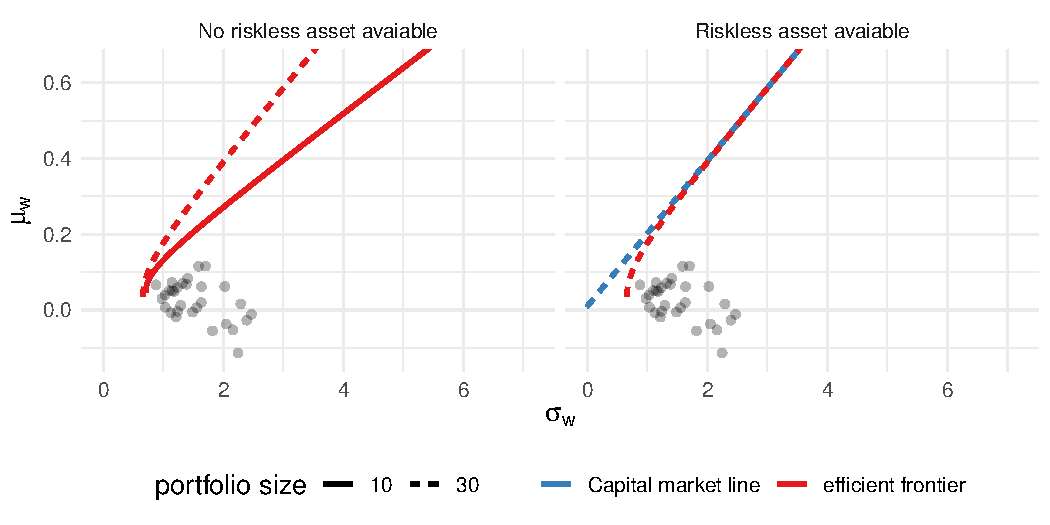
\includegraphics[width=\maxwidth]{figure/mertons_efficient_frontier-1} 

}

\caption[Efficient frontiers with and without a risk-free asset]{Efficient frontiers with and without a risk-free asset. The left plot illustrates two different efficient frontiers for different portfolio sizes. The right plot we illustrate the efficient frontier and the capital market line which appears when a riskless asset is available. The stocks are randomly selected from the S\&P500. The individual means and standard deviations are displayed as points.}\label{fig:mertons_efficient_frontier}
\end{figure}

\end{knitrout}
Any point on any of the two lines in the left hand-side plot of Figure \ref{fig:mertons_efficient_frontier} corresponds to a certain efficient and optimal portfolio with a specific value of $\mu_0$. 
The points in the two plots depicts the expected returns and the standard deviations of a single-stock portfolio. 
You can obtain these by investing in everything you got in a specific stock. 
However, diversification will always decrease the risk we take which can be seen in the illustration. 
No single-stock portfolio can outperform any of the portfolios on the efficient frontier. 
That can not happen. 
The efficient frontier is the best we can do with the stocks at hand, given the objective.

The right hand-side plot of Figure \ref{fig:mertons_efficient_frontier}, displays an extension to the mean-variance problem.
It displays what happens when we include a risk-free asset in the portfolio allocation problem. 
To introduce this option into our allocation problem we add the risk-free rate as part of the portfolio $w_0 r_f + \bw^\top \bx$ and optimize over $w_0$ as well. 
We assume that the risk-free rate is deterministic and therefore \eqref{eqn:mean_variance} becomes 
\begin{equation}\label{eqn:mean_variance_riskfree}
\begin{aligned}
& \underset{\bw}{\text{minimize}} 
& & \bw^\top \bSigma \bw \\
& \text{subject to}
& & w_0 + \bw^\top \ones = 1 \\
& && w_0 r_f + \bw^\top \bmu = \tilde\mu_0 \\
\end{aligned}
\end{equation}
However, since $w_0 + \bw^\top \ones=1$ we substitute $w_0=1-\bw^\top \ones$ and solve the unconstrained optimization problem instead. 
Its solution is given by 
\begin{equation}\label{eqn:w_mean_variance_riskfree}
  \bw_{TP} = \frac{(\tilde\mu_0-r_f)}{(\bmu-r_f \ones)^\top \bSigma^{-1} (\bmu-r_f \ones)} \bSigma^{-1} (\bmu-r_f \ones).
\end{equation}
The collection of portfolios given by \eqref{eqn:mean_variance_riskfree} defines the whole capital market line which is shown in Figure \ref{fig:mertons_efficient_frontier}. 
The portfolio has many interesting properties. 
If there is a risk-free asset, then we can increase the return and decrease the risk of our position in the market. 
This is most easily explained by the efficient frontier, displayed in Figure \ref{fig:mertons_efficient_frontier}. 
For a given level of risk we can sometimes get the same or large return! 
The same solution can be obtained from the optimization problem with the quadratic utility, defined as 
$$\min_{\bw} \bw^\top \bmu - \frac{\gamma}{2} \bw^\top \bSigma \bw$$ 
for some $\gamma > 0$.
The solution is given by 
$$\frac{1}{\gamma}\bSigma^{-1} (\bmu-r_f \ones)$$
which coincide with \eqref{eqn:w_mean_variance_riskfree} if 
$$\frac{1}{\gamma} = \frac{(\tilde\mu_0-r_f)}{(\bmu-r_f \ones)^\top \bSigma^{-1} (\bmu-r_f \ones)}.$$ 
The difference is that \eqref{eqn:w_mean_variance_riskfree} depends on a number of parameters while $\gamma$ is a fixed constant.
This is quite common in MPT, there are many portfolio allocation problems which result in the same solution, see e.g. \citet{bodnar2013equivalence}.

Ever since the end of 2014, there has been a lack of a risk-free asset in Sweden.\footnote{See \href{https://www.riksbank.se/sv/statistik/sok-rantor--valutakurser/reporanta-in--och-utlaningsranta/}{this visualization from Riksbanken}} 
The risk-free rate has been equal to or less than zero. 
Assuming that is true for our hypothetical investor, \eqref{eqn:w_mean_variance_riskfree} reduces to $\bw_{TP} = \tilde\mu_0 \bSigma^{-1} \bmu / \bmu^\top \bSigma^{-1} \bmu$. 
The term $\bSigma^{-1} \bmu$ is also present in \eqref{eqn:mean_var_solution}, although hidden with the introduction of the matrix $\bQ$. 
With a little work, one can rewrite \eqref{eqn:mean_var_solution} as
$$
\left(1 - \frac{\mu_0-\R}{\V^2} \R \right) \bw_{GMV} + \frac{\mu_0-\R}{\V} \bSigma^{-1} \bmu.
$$
There are two insights to be drawn from this equation. 
The first is that the weights on the efficient frontier is a combination of two portfolios, in this case the GMV and the tangency portfolio. 
This result is usually known as the Mutual fund theorem, see \textcite{tobin1958liquidity}.
To study all the portfolios on the efficient frontier we only need to study these two portfolios. 
The second is that the true tangency portfolio is given by \eqref{eqn:w_mean_variance_riskfree} with 
$$
\tilde\mu_0 = \R + \frac{\mu_0-\R}{\V} s  
$$
which is where the efficient frontier and the capital market line meet. 
Any tangency portfolio with $\mu_0\leq \R + \frac{\mu_0-\R}{\V} s$ will be "more efficient" than the efficient frontier if there is a risk free rate. 
However, its not always the case that we want to optimize the amount of cash held in the risk-free asset. 
Given that cash is free, we should most likely borrow as much as possible to invest in the market which might be a risk in itself.

All of MPT use the inverse covariance matrix. In the next section we devote some attention to the assumption we make on the covariance matrix.  

\section{Relationship between assets and the (inverse) covariance matrix}\label{subsec:cov_prec_matrix}
%%% ----------------------
The covariance matrix $\bSigma$ and the precision matrix $\bSigma^{-1}$ are fundamental to mean-variance portfolio theory. 
In this section we discuss the restrictions we place on the covariance matrix and what the precision matrix actually represent. 

For a vector $\by$ with finite second moment, the covariance matrix is defined as $\bSigma=\optn{E}((\by - \bmu)(\by - \bmu)^\top)$. 
It contains the variances of each individual element of $\by$ on the diagonal as well as the covariances between every pair of elements on the off-diagonal. 
That is, each diagonal element corresponds to the univariate case with variance equal to $\optn{E}((y_i - \mu_i)^2)$. 
In the univariate case, a distribution is usually called degenerate or singular if the variance is equal to zero. 
In the multivariate case. the covariance matrix can be singular on a number of occasions. 
It is not limited to the diagonal elements.
This is due to the fact that we involve covariances on the off-diagonal and we are therefore forced to work with a broader definition.  
Since we work with real matrices in this thesis, we limit the definition accordingly. 
From \textcite[ch 14.2]{harville1997matrix} we say that a real symmetric $p\times p$ matrix $\bA$ is called 
\begin{itemize}
	\item positive definite if $\bz^\top \bA \bz > 0$
	\item positive semi-definite if $\bz^\top \bA \bz \geq 0$
\end{itemize}
for all nonzero vectors $\bz \in \mathbbm{R}^p$.
We will use $\bA > 0$ or $\bA \geq 0$ to indicate positive or semi-positive definiteness of the matrix $\bA$. 
In the multivariate case we need to assert that a quadratic form is (strictly) positive to assert if the distribution is degenerate or not. 
The definition of positive- or semi-positive definiteness can be quite cumbersome to work with. 
We need to assert that the conditions holds for all vectors $\bz$. 
One necessary condition for a matrix to be positive definite can be derived using the eigenvalues of a matrix and its eigenvalue decomposition, as described in \textcite[ch. 21]{harville1997matrix},
\begin{definition}\label{def:eigenvalue} 
	Let $\bA$ be a $p\times p$ matrix. The characteristic roots (with multiplicity) are given by the solutions to
	\begin{equation*}
		\left|\bA - \lambda \bI\right| = 0
	\end{equation*}
	where $|\cdot|$ is the determinant of a matrix.
\end{definition} 
Let $\lambda_i$, $i=1,2,...,p$, denote the \textit{ordered} eigenvalues of the matrix $\bA$ such that $\lambda_1\geq \lambda_2 \geq ... \geq \lambda_p$.
Given an eigenvalue, the eigenvectors $\bu_i$ are defined by $\bA \bu_i = \lambda_i \bu_i$, $i=1,2,...,p$. 
Let $\boldsymbol{\Lambda} = \operatorname{diag}(\lambda_1, \lambda_2,...,\lambda_p)$ and $\bU= (\bu_1^\top, \bu_2^\top, ..., \bu_p^\top)^\top$. 
It might happen that eigenvalues are equal, such as when $\bSigma = \sigma \bI$.
Using the relation between eigenvalues and their eigenvectors we can derive the eigenvalue (or spectral) decomposition of a symmetric matrix 
\begin{equation}\label{eqn:eigenvalue_decomp}
	\bA = \bU \boldsymbol{\Lambda} \bU^{-1}.
\end{equation}
Since $\bA$ is symmetric it also holds that $\bU^{-1} = \bU^\top$.
A necessary condition for a matrix to be positive definite can be directly obtained from the eigenvalue decomposition. 
Let $\bz\in \mathbbm{R}^p$ and $\by := \bU^{\top} \bz \in \mathbbm{R}^p$, then $\bz^\top \bA \bz = \bz^\top \bU \boldsymbol{\Lambda} \bU ^{\top} \bz = \by^\top \boldsymbol{\Lambda} \by = \sum_i^p \lambda_i y_i^2$ which is a second degree polynomial. 
If the eigenvalues are all positive, then necessarily the matrix is positive definite. 
If there are some eigenvalues which are zero then the matrix is semi-positive definite. 

In all papers of this thesis we assume that the true covariance matrix is positive definite. 
The assumption has a deep economical interpretation.
If one (or more) eigenvalue(s) are zero then there is a possibility to construct a portfolio which does not contain any risk with a potentially positive return. 
Its an arbitrage opportunity unless the elements of $\bmu$ are all zero.
Assume $\lambda_p=0$, let $\bu_p$ be its eigenvector and set $\bw = \bu_p / \sum_i^p u_{ip}$. 
The variance of that portfolio is zero since all eigenvectors are orthonormal and its mean is $\bw^\top \bmu$.
If the true covariance matrix is not positive definite there might exist arbitrage opportunities, e.g. the possibility of making profit without taking any risk.

%The eigenvalue decomposition is very useful.
%%It provides a simple way to construct inverses, which is very important for MPT as seen in \eqref{eqn:mean_var_solution}.
%We claim that $\bB = \bU \boldsymbol{\Lambda}^{-1} \bU^{-1}$ is a valid inverse which is easy to verify since $\bB \bA = \bU \boldsymbol{\Lambda}^{-1} \bU^{-1} \bU \boldsymbol{\Lambda} \bU^{-1} = \bI$. 
%To study the inverse of the covariance matrix we can study the eigenvectors and the inverse of its eigenvalues.
%Secondly, it contains a lot of information that might not be available at first glance. 
%If $\bA$ is a covariance matrix then it contains variances and covariances, describing relations between random variables. 
%The eigenvectors are rotations that try to capture as much variation as possible along its axis.
%The eigenvalues is the variation along the eigenvectors axis. 
%They describes how the system behaves and not the individual elements and their inverse values describe how the precision matrix behaves.

%%%%%% ------------------------------------------------------------------------
\chapter[Models \& inference]{Statistical models and inference}\label{ch:estim}
%%%%%% ------------------------------------------------------------------------


To \textit{pratically} use the portfolios described by \eqref{eqn:mean_var_solution} we have to specify the two parameters $\bmu$ and $\bSigma$. 
This is not really feasible if we have many assets. 
We might have an opinion of what they should be, however we do not know them precisely.  
Furthermore, even if one has an informed opinion of the parameters $\bmu$ and $\bSigma$, the potential loss of using those exact parameters might be paramount. 
We usually want to rely on data to estimate the parameters of interest.
In this thesis we never use the asset prices themselves but a transformation of the relative differences, that is, their simple and log-returns. 
Let $p_{i,t}$ be the asset price of the $i$th asset at time $t$. 
The simple return is defined as $r_{i,t} := (p_{i,t}-p_{i,t-1})/p_{i,t-1}$ and the log-return is then defined as $y_{i,t} := \log(r_{i,t} + 1)$ and $\by_t=(y_{1,t},y_{2,t},..., y_{p,t})$.
The return of a portfolio with $p$ assets is modeled as $\bw^\top \by_t$ where $\bw=(w_1, ..., w_p)$ are the portfolio weights.
Notice that this is an approximation. 
In reality we would want to work with $\sum_{i=1}^p w_i r_{i,t}$ (or even $\sum_{i=1}^p w_i p_{i,t}$) since it is additive in the number of assets.
However, logarithmic returns are additive in time which can be desirable. 
Compounding returns is simple addition and the approximation can make the statistical analysis more tractable. 
The difference between the two approaches is very small if the (log) returns are small, which is often true for financial assets, see \citet[p. 5]{tsay2005analysis}. 

Assuming that we have a model for the log-returns there are many ways of estimating $\bmu$ and $\bSigma$.
The most simple and versatile method is the method of moments (MM) (see e.g. \citet[ch. 9]{wasserman2004all}). 
Let $\bY = (\by_1, \by_2, ..., \by_n)$ be a sample of log-returns.
Using the sample, we replace $\bmu$ with the sample mean and $\bSigma$ with the sample covariance matrix, i.e.
$$
\byb = \frac{1}{n} \sum_i^n \by_i, \; \bS = \frac{1}{n}\bY \left(\bI_n - \frac{1}{n} \ones_n \ones_n^\top \right) \bY^\top.
$$
This is always a feasible approach assuming that the first two moments actually exist. 
However, it introduces some issues.
If our sample size $n$ is small, then our estimates are naturally imprecise. 
Furthermore, MPT relies on $\bS^{-1}$ and not $\bS$.
It demands that $n>p$. 
Its natural to ask: does an imprecise estimate of the covariance matrix provide an equally imprecise estimate of the inverse?
In some simple cases the answer is no, sometimes its worse. 
It is therefore very important to understand the implications of not using the true parameters but their sample counterparts.
There are many approaches to this but we take the bottom-up approach. 
If we assume that the asset returns $\bY$ follow some distribution then we can perhaps derive statistical properties for $\byb$ and $\bS$.
In turn, we need to derive the properties of $\bS^{-1}$ and in the end all the transforms given by \eqref{eqn:mean_var_solution}.
In the coming sections we state the models used in this thesis and some important properties thereof.
We thereafter discuss the implications for MPT.

\section{Matrixvariate distributions}
One of the most fundamental models for asset returns is the multivariate normal distribution. 
Since most of the distributions we work with are matrix variate, we will state the matrixvariate normal distribution. 
It is slightly more general but it can capture much more dynamics.
% Multivariate normal distribution
\begin{definition}[Definition 2.2.1 \citet{GuptaNagar2000}]\label{def:matrixnormal}
	The random matrix $\bY$ $(p \times n)$ is said to have a matrix variate normal distribution with mean matrix $\bM$ and covariance matrix $\bSigma \otimes \bGamma$ where $\bSigma > 0$ is of dimension $(p \times p)$ and $\bGamma >0$ is of dimension $(n \times n)$, if $\optn{vec}(\bY^\top) \sim N_{np}(\optn{vec}(\bM^\top), \bSigma \otimes \bGamma)$.
\end{definition}
The multivariate normal distribution is a simple special case of it with $\bGamma = \bI$ and $n=1$.
This model is used very often and the applications are many. 
However, \citet{cont2001empirical} describes a number of stylized facts of log-returns. 
These stylized facts describes the characteristics asset returns on different frequencies.  
It is argued that the multivariate normal distribution has to thin tails in comparison to what is usually observed in asset returns on higher frequencies.
He argues that daily returns are usually not symmetric and often show volatility clustering.  
However, he also argues that returns on a lower frequency such as monthly or quarterly can be close to normal.
The shape of the unconditional return distribution is not the same over different frequencies. 
A motivation for the multivariate normal model can be thought of as an investor which invests or rebalance their portfolio infrequently.
That does not mean that they cannot observe the results of the market on a higher frequency than they invest!

In the univariate case we have that the sample variance follows a chi-square distribution. 
If the returns follow a multivariate normal distribution and are independent, then $\bS$ follows what is known as a Wishart distribution. 
It is essentially a generalization of the chi-square distribution. 
We state its probability density function (p.d.f.) below.
% Wishart
\begin{definition}[Definition 3.2.1 \citet{GuptaNagar2000}]\label{def:wishart}
	A $p\times p$ random symmetric positive definite matrix $\bS$ is said to have a Wishart distribution with parameters $p, n$ ($n\geq p$) and $\bSigma > 0$, $(p \times p)$ written as $\bS \sim W_p(n, \bSigma)$ if its p.d.f. is given by
	\begin{equation}\label{eqn:wishart_density}
  	\frac{|\bS|^{(n-p-1)/2} |\bSigma|^{- n/2} }{2^{pn/2} \Gamma_p (n/2) } \exp\left\{-\frac{1}{2} \operatorname{tr}(\bSigma^{-1}\bS)  \right\}
	\end{equation}
	where $ \Gamma_p (\cdot) $ is the multivariate gamma function.
\end{definition}
In comparison to the normal distribution the Wishart distribution is used very frequently as a model for covariance matrices although in a slightly different context.
The model is very often used for realized covariance matrices, see \citet{barndorff2004econometric}, \citet{golosnoy2019exponential} or \citet{alfelt2021modeling}.
A realized covariance matrix is an estimates of the volatility process from returns on a much higher frequency than we work with in this thesis.
From Theorem 3.3.6 we know that if $\bY \sim N_{p,n}(\bmu \ones_n^\top, \bSigma \otimes \bI_n)$, then $n\bS \sim W(n-1, \bSigma)$, so working from the bottom up we can get a model for the parameters of the model.
As previously stated, MPT works with inverse covariance matrices and not with the covariance matrix itself. 
Thankfully, the Wishart distribution has an inverse counterpart.
% Inverse Wishart
\begin{definition}[Definition 3.4.1  \citet{GuptaNagar2000}]\label{def:inverse_wishart}
	A random matrix $\bV$ is said to be distributed as an inverted Wishart distribution with $m$ degrees of freedom and parameter matrix $\bGamma$ $(p \times p)$, denoted by $\bV \sim IW_p(m, \bGamma)$, if its density is given by
	\begin{equation}\label{eqn:inverse_wishart}
	\frac{2^{-(m-p-1)p/2} |\bGamma|^{(m-p-1)/2} }{\Gamma_p ((m-p-1)/2) |\bV|^{m/2}} \exp\left\{ -\frac{1}{2} \bV^{-1} \bGamma \right\}, \; m > 2p, \bV, \bGamma > 0.
	\end{equation}
\end{definition}
To once more connect to the univariate setting, the inverted sample variance follows an inverted chi-square distribution which is a special case of the inverted gamma distribution.
It is only natural that the inverted Wishart matrix is a matrix variate generalization of the inverted gamma distribution (p. 111 \citet{GuptaNagar2000}). 
It demands quite specific constraints on the parameters of the model, namely $m > 2p$.
To come back to out question we posed in the beginning of this section, does the inverse change uncertainty? 
We can at least get a hint that \textit{something} changes with the properties of $\bS$ when taking inverses.
The constraints of the model are more strict.
From Theorems 3.3.7 and 3.4.1, and Theorem 3.4.3 of \citet{GuptaNagar2000} we have that
$$
\optn{E}\left[\bS\right] = \frac{n-1}{n} \bSigma, \; 
\optn{E}\left[\bS^{-1}\right] = \frac{n}{n-p-2}\bSigma^{-1}.
$$
If $n$ is sufficiently large, than the sample covariance matrix is (close to) unbiased.
That is not necessarily the case for its inverse.
If we believe in diversification then we should own many assets, e.g., $p$ should be large. 
That in turn could make the estimator very biased!
The answer is yes, inverses can potentially make matters worse.
Furthermore, the noise in the sample mean can be extremely large in comparison to the noise in the sample covariance matrix.
The weights from \eqref{eqn:mean_var_solution} will be much more noisy whenever $\mu_0 \neq \R$ since these will depend on the sample mean vector (see e.g. \citet{merton1980estimating}, \citet{chopra1993effect}).
It is perhaps one of the most common motivations for using the GMV portfolio.

It has been well established that for higher frequency returns the normal assumption is limiting. 
The next, and perhaps most common feature, to include is skewness of the asset returns and to assess its effect on portfolios. 
A $p$ dimensional Closed Skew Normal (CSN) random vector $\bz$ has density
\begin{equation}
  f_\bz(\ba; \bmu, \bSigma, \bD, \bv, \Delta) = C \phi_p(\ba; \bmu, \bSigma) \Phi_q(\bD(\ba-\bmu); \bv, \Delta)
\end{equation}
where $C$ is a normalization constant and $\bmu, \bSigma, \bD, \bv$ and $\Delta$ are parameters of appropriate dimensions. Its matrix variate counterpart is simply defined through the vec operator. We have that
% Closed skew normal distribution
\begin{definition}[Definition 3.1 \citet{dominguez2007matrix}]
  A random matrix $\bY$ $(p \times n)$ is said to have a matrix variate closed skew-normal distribution with parameters $\bM$ $(p \times n)$, $\bA$ $(np \times np)$, $\bB$ $(nq \times mp)$, $\bL$ $(q \times m)$ and $\bQ$ $(mq \times mq)$, with $\bA > 0$ and $\bQ>0$ if
  \begin{equation}
    \optn{vec}(\bY^\top) \sim CSN_{pm, qn}\left(\optn{vec}(\bM^\top), \bA, \bB, \optn{vec}(\bL^\top), \bQ\right)
  \end{equation}
\end{definition} 
The closed skew-normal distribution is heavily parametrized. 
For each column in the matrix $\bY$  we have a mean vector $\bm$ and an additional four vectors $\ba$, $\bb$, $\bl$ and $\bq$ describing skewness and volatility of the asset returns.
The matrixvariate distribution can capture a lot of dynamics.
However, it also puts a heavy restriction on some of the parameters, as they need to be positive definite.
The parameter $\bA$ might be interpreted as a covariance matrix although that is a simplification.
It is something more.
It can capture variance along \textit{both} axis of the matrix $\bY$, such as volatility for a specific asset but also unconditional volatility over time.
There is also some type of dependence between $\bA$ and how skewness is observed, by the fact that moments include \textit{almost all of the parameters} (see e.g. Proposition 3.2 \citet{dominguez2007matrix}).
From the stochastic representation in Proposition 2.1 \citet{dominguez2007matrix} one can, after some thought and derivations
\footnote{The proposition is a little bit misleading as there seems to be an absolute value missing and the parameter $\bv$ appears as random but is also part of the parametrization. To arrive at the correct representation, the reader can go through the steps that begins at the end of page 7 in the same reference (page 1606).}
realize that the skewness is introduced as shocks to the mean.
The mean is stochastic.
The overzealous parametrisation and difficulty in estimating the parameters made us choose a special case of it for paper 2 of this thesis.
We work with a special case of the distribution where $q=m=1$.

% 
The last model we consider in this thesis is the most general.
It is also the model that has the least amount of interesting properties in itself.
It is the following location and scale model
\begin{equation}\label{eqn:location_scale_model}
\bY \eqdist \bmu \ones^\top_n + \bSigma^{1/2} \bZ.
\end{equation}
where $\eqdist$ stands for equality in distribution and $\bZ = \{z_{ij}\}$, $i=1,2,...,p$, $j=1,2,...,n$.
Although the model can capture many types of return distributions, such as skew heavy tailed sometimes even heteroscedasticity, there is very little to say about it.
In this thesis we very often assume moment conditions on the "residuals" $z_{ij}$ such as finite fourth moment or potentially $4+\epsilon$ finite moment, for some $\epsilon>0$.
The difference between finite fourth moment and $4+\epsilon$ is most often the claims of convergence we can show.
With the slightly more stringent assumption we can make claims about almost sure convergence and with finite fourth we can usually make claims about convergence in probability (see the supplement material of \citet{BodnarGuptaParolya2016}).

\section{Inference and sampling distributions of optimal portfolios and their characteristics}
Replacing $\bmu$ and $\bSigma$ with $\byb$ and $\bS$ in \eqref{eqn:mean_var_solution} we get its empirical counterpart
\begin{equation}\label{eqn:meanvar_solution_sample}
	\hbw_{MV} = \frac{\bS^{-1}\ones}{\ones^\top \bS^{-1}\ones} + \frac{\mu_0 - \hR}{\hV} \hat{\bQ} \byb,\; \hat{\bQ} = \bS^{-1} - \frac{\bS^{-1} \ones \ones^\top \bS^{-1}}{\ones^\top \bS^{-1} \ones}
\end{equation}
where 
\begin{equation}\label{eqn:meanvar_characteristics_sample}
  \hV = \frac{1}{\ones^\top \bS^{-1}\ones},\; \hR = \frac{\ones^\top \bS^{-1} \byb}{\ones^\top \bS^{-1}\ones}
\end{equation}
and the shape parameter of the efficient frontier $\hat{s} = \byb^\top \bQ \byb$.
This is a portfolio we can actually invest in. 

From the previous section we know the distributions of $\byb$ and $\bS$ if $\bY$ follows distribution stated in Definition \ref{def:matrixnormal}. 
In this scenario the two parameters are independent (see Theorem 3.3.6 \citet{GuptaNagar2000}) which makes the analysis simpler.
However, there are many complicated transforms containing both $\byb$ and $\bS^{-1}$.
One example is the weights for the GMV portfolio
$$
\hbw_{GMV}=\frac{\bS^{-1}\ones}{\ones\bS^{-1}\ones}.
$$
It contains the sample covariance matrix in the nominator as well as the demoniator.
Its not safe to assume that these are independent nor is it trivial to state when they would be.
To solve the problem at hand consider two $p\times p$ matrices with the following block structure 
\begin{equation}\label{eqn:blockmat}
\bA = \begin{pmatrix}
       \bA_{11} & \bA_{12} \\
       \bA_{21} & \bA_{22}
      \end{pmatrix},\;
\bV = \begin{pmatrix}
           \bV_{11} & \bV_{12} \\
           \bV_{21} & \bV_{22}
          \end{pmatrix}
\end{equation}
where $\text{dim}(\bA_{11}) = \text{dim}(\bV_{11})= m \times m$, $m<p$. 
Let $\bA_{11\cdot 2} := \bA_{11} - \bA_{12} \bA_{22}^{-1} \bA_{21}$ denote the Schur complement of the matrix $\bA$ and define $\bV_{11\cdot 2}$ in the same manner. 
Let $\otimes$ denote the Kronocker product. 
The following theorem is used a lot in papers 1 and 2.
\begin{theorem}[Theorem~3 in \citet{BodnarOkhrin2008}]\label{thrm:invWis}
 Suppose $\bA \sim W^{-1}_k(n, \bV)$, where $\bA$ and $\bV$ are partitioned as in \eqref{eqn:blockmat}. Then
 \begin{enumerate}[(a)]
	\item $\bA_{11\cdot 2} \sim W^{-1}_m(n-k+m, \bV_{11\cdot 2})$ and is independent of $\bA_{22}$;
 	\item $\bA_{12} | \bA_{22}, \bA_{11\cdot 2} \sim \mathcal{N}(\bV_{12}\bV^{-1}_{22} \bA_{22}, \bA_{11\cdot 2} \otimes \bA_{22} \bV^{-1}_{22} \bA_{22})$;
	\item $\bA_{22} \sim W^{-1}_{p-m} (n-2m, \bV_{22})$;
	\item $\bA_{12}\bA^{-1}_{22}$ is independent of $\bA_{22}$, with density given by 
	\begin{flalign}
            f_{\bA_{12}\bA^{-1}_{22}}(\bX) = & \frac{  |\bV_{11\cdot 2}|^{-\frac{1}{2} (p-m)} |\bV_{22}|^{\frac{1}{2}m}  }{ \pi^{\frac{(p-m)m}{2}} } \frac{\Gamma_{m} \left(\frac{n-m-1}{2} \right)}{\Gamma_{m} \left(\frac{n-p-1}{2} \right)} \nonumber \\
            & \times \left|\bI + \bV^{-1}_{11\cdot 2} \left(\bX - \bV_{12}\bV_{22}^{-1} \right)\bV_{22} \left(\bX - \bV_{12}\bV_{22}^{-1} \right)^\top  \right|^{-\frac{1}{2}(n-m-1)} \label{eqn:almostT}
	\end{flalign}
	where $\Gamma_{m}(\cdot)$ is the multivariate Gamma function;
	\item $\bA_{22}$ is independent of $\bA_{12}\bA^{-1}_{22}$ and $\bA_{11\cdot 2}$;
	\item $\bA_{11\cdot 2}| \bA_{12}\bA^{-1}_{22}=\bX \sim W_m^{-1}(n,  \bV_{11\cdot 2} + \left(\bX - \bV_{12}\bV_{22}^{-1} \right)\bV_{22} \left(\bX - \bV_{12}\bV_{22}^{-1} \right)^\top )$
 \end{enumerate}
\end{theorem}
So given a inverse Wishart distribution we can derive the distribution of many, quite difficult, transformations of its sub-matrices. 
Let $\bM^\top = (\bL^\top , \ones^\top)$ and note that $(\bM \bS^{-1} \bM^\top)^{-1}$ follows a Wishart distribution by Theorem 3.3.13 \citet{GuptaNagar2000}. 
We can then invert $(\bM \bS^{-1} \bM^\top)^{-1}$, use the fact that the inverse of a Wishart matrix follows an inverse Wishart distribution and at last use the fact that 
$$
\bM \bS^{-1} \bM^\top = 
\begin{pmatrix}
\bL^\top \bS^{-1} \bL & \bL^\top \bS^{-1} \ones \\
\ones^\top \bS^{-1} \bL^\top & \ones^\top \bS^{-1} \ones \\
\end{pmatrix}.
$$
Its then easy to see that
$$
\bA_{12}\bA^{-1}_{22}= frac{\bL^\top \bS^{-1} \ones}{\ones^\top \bS^{-1} \ones}
$$
By \eqref{eqn:almostT} we can find the density of the GMV portfolio. 
Furthermore, we can actually assert that the GMV portfolio weights and the variance of the GMV portfolio are independent!
Paper 1 use these properties to derive the full joint distribution for all the quantities used in \eqref{eqn:meanvar_solution_sample}.
The result is more general than that as we derive the distribution of all optimal portfolios but since the classical mean-variance portfolio is one of them we get that for free. 
The joint distribution is characterized through its stochastic representation.
The stochastic representation is a very verbose way of characterizing the distribution in terms of simple random variables.
These random variables are simple to simulate.
To compute any quantity of interest from the joint distribution we can simply compute it through monte carlo approximation. 
For some methods simulations are the only way we can compute the quantities of interest.
It can therefore be very important that simulations are fast.
This is extremely simple to do when you have the stochastic representation.

\section{Simulations, inverses and why stochastic representations are valuable}
Assume that the investor cares about simulations, is interested in the GMV portfolio and for the train of thought that $\bY \sim N_{p,n}(\bmu \ones_n^\top, \bSigma \otimes \bI_n)$. 
To simulate from the sampling distribution of the variance of the GMV portfolio we need to 
\begin{enumerate}
  \item Simulate $\bY$ and construct $\bS$
  \item Invert $\bS$
  \item Compute $\hV$
\end{enumerate}
The second step is notoriously demanding.
The default method to use in R is \hlstd{solve} which is a wrapper for certain LAPACK\footnote{For the interested reader \url{https://www.netlib.org/lapack/}} functions.
The inverse itself takes $2p^3$ flops (cpu cycles), which is not cheap (see e.g. \citet[ch 14]{higham2002accuracy}).
If $p$ is large then simulation of the quantity $\hV$ will be extremely cumbersome.
Another method is R's \hlstd{chol2inv} which relies on the Cholesky decomposition. 
In theory it should be faster but demands that we compute the Cholesky decomposition.
The last two options that are available is to simulate $\bS$ directly or to derive the stochastic representation of $\hV$ directly.
Paper 1 and 2 goes into great detail to derive the stochastic representation of different quantities of optimal portfolios. 
One of them is the sample variance of the GMV portfolio.
By Theorem 1 in \citet{bodnar2020sampling} we know that if $\bY \sim N_{p,n}(\bmu \ones_n^\top, \bSigma \otimes \bI_n)$, then $\hV \sim \V\xi /(n-1)$ where $\xi \sim \chi^2_{n-p}$.
We can omit inversions all together.
In \ref{benchmark} we present R-code which implements a small benchmark to highlight why these types of representations can be really valuable.
\begin{knitrout}\small
\definecolor{shadecolor}{rgb}{1, 1, 1}\color{fgcolor}\begin{kframe}
\captionof{chunk}{R-code for benchmarking different simulation approaches of the variance of the GMV portfolio.}\label{benchmark}\begin{alltt}
\hlcom{# setup}
\hlstd{p} \hlkwb{<-} \hlnum{150}
\hlstd{n} \hlkwb{<-} \hlnum{250}
\hlstd{Sigma} \hlkwb{<-} \hlstd{HDShOP}\hlopt{::}\hlkwd{RandCovMtrx}\hlstd{(p)}
\hlstd{Sigma_chol} \hlkwb{<-} \hlkwd{chol}\hlstd{(Sigma)}
\hlstd{mu} \hlkwb{<-} \hlkwd{runif}\hlstd{(p,} \hlopt{-}\hlnum{0.1}\hlstd{,} \hlnum{0.1}\hlstd{)}
\hlstd{Sigma_inv} \hlkwb{<-} \hlkwd{solve}\hlstd{(Sigma)}
\hlstd{V_GMV} \hlkwb{<-} \hlnum{1}\hlopt{/}\hlkwd{sum}\hlstd{(Sigma_inv)}
\hlcom{# microbechmark}
\hlstd{result} \hlkwb{<-} \hlkwd{microbenchmark}\hlstd{(}
  \hlcom{# Simulate Y directly, construct S, invert and compute GMV variance}
  \hlkwc{`Scenario 1`} \hlstd{= \{}
    \hlstd{Y} \hlkwb{<-} \hlstd{mu} \hlopt \hlkwd{t}\hlstd{(}\hlkwd{rep}\hlstd{(}\hlnum{1}\hlstd{,n))} \hlopt{+} \hlkwd{t}\hlstd{(Sigma_chol)}\hlopt\hlkwd{matrix}\hlstd{(}\hlkwd{rnorm}\hlstd{(n}\hlopt{*}\hlstd{p),} \hlkwc{ncol} \hlstd{= n)}
    \hlstd{S} \hlkwb{<-} \hlkwd{var}\hlstd{(}\hlkwd{t}\hlstd{(Y))}
    \hlnum{1}\hlopt{/}\hlkwd{sum}\hlstd{(}\hlkwd{solve}\hlstd{(S))}
  \hlstd{\},}
  \hlcom{# Simulate Y directly, construct S and its chol. decomp., use chol2inv and}
  \hlcom{# compute GMV variance}
  \hlkwc{`Scenario 2`} \hlstd{= \{}
    \hlstd{Y} \hlkwb{<-} \hlstd{mu} \hlopt \hlkwd{t}\hlstd{(}\hlkwd{rep}\hlstd{(}\hlnum{1}\hlstd{,n))} \hlopt{+} \hlkwd{t}\hlstd{(Sigma_chol)}\hlopt\hlkwd{matrix}\hlstd{(}\hlkwd{rnorm}\hlstd{(n}\hlopt{*}\hlstd{p),} \hlkwc{ncol} \hlstd{= n)}
    \hlstd{S} \hlkwb{<-} \hlkwd{var}\hlstd{(}\hlkwd{t}\hlstd{(Y))}
    \hlstd{S_chol} \hlkwb{<-} \hlkwd{chol}\hlstd{(S)}
    \hlnum{1}\hlopt{/}\hlkwd{sum}\hlstd{(}\hlkwd{chol2inv}\hlstd{(S_chol))}
  \hlstd{\},}
  \hlcom{# Simulate S directly, invert and compute GMV variance}
  \hlkwc{`Scenario 3`} \hlstd{= \{}
    \hlstd{S} \hlkwb{<-} \hlkwd{rWishart}\hlstd{(}\hlnum{1}\hlstd{,} \hlkwc{df}\hlstd{=n}\hlopt{-}\hlnum{1}\hlstd{,} \hlkwc{Sigma}\hlstd{=Sigma)[,,}\hlnum{1}\hlstd{]}
    \hlnum{1}\hlopt{/}\hlkwd{sum}\hlstd{(}\hlkwd{solve}\hlstd{(S))}
  \hlstd{\},}
  \hlcom{# Simulate directly from the GMV sample variance distribution.}
  \hlkwc{`Scenario 4`} \hlstd{= V_GMV}\hlopt{/}\hlstd{(n}\hlopt{-}\hlnum{1}\hlstd{)} \hlopt{*} \hlkwd{rchisq}\hlstd{(}\hlnum{1}\hlstd{,} \hlkwc{df}\hlstd{=n}\hlopt{-}\hlstd{p),}
  \hlkwc{times}\hlstd{=}\hlnum{1000}
\hlstd{)}
\end{alltt}
\end{kframe}
\end{knitrout}

\begin{knitrout}\small
\definecolor{shadecolor}{rgb}{1, 1, 1}\color{fgcolor}\begin{figure}

{\centering 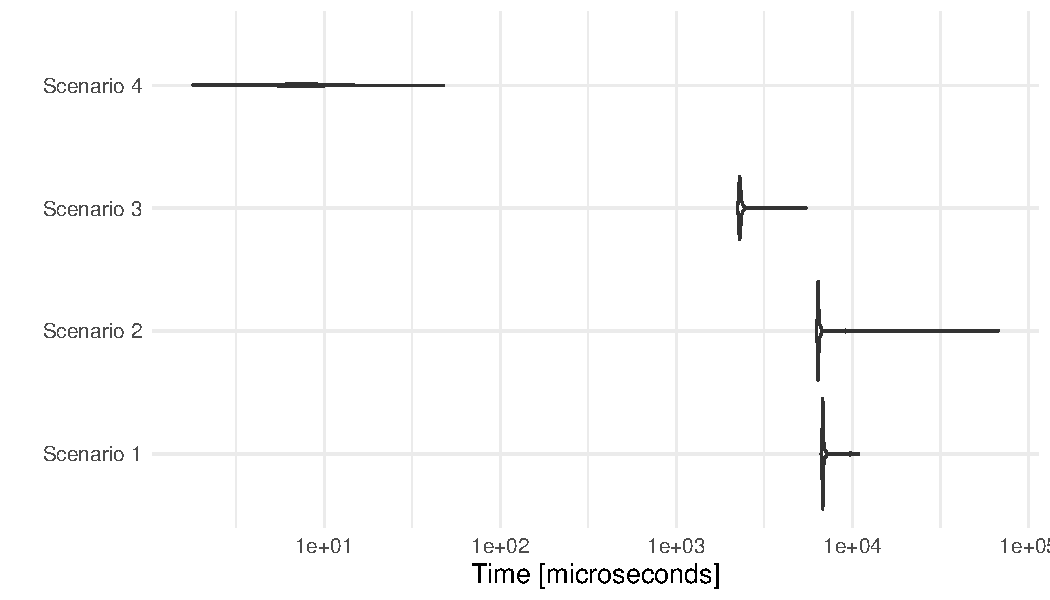
\includegraphics[width=\maxwidth]{figure/microbenchmark_output-1} 

}

\caption[Difference in performance between the simulation methods for the estimated variance of the GMV portfolio based on 1000 simulations]{Difference in performance between the simulation methods for the estimated variance of the GMV portfolio based on 1000 simulations.}\label{fig:microbenchmark_output}
\end{figure}

\end{knitrout}

Scenario 4 uses the stochastic representation. 
The execution time of scenario 4 is much smaller than the former strategies.
It is quite clear that it is the fastest. 
The conclusion is that inversions are very cumbersome to deal with and take a lot of time regardless if we use the Cholesky decomposition or not.
Its can also be a very unstable operation, especially if the matrix you are trying to invert is close to singular.

So far we have assumed that all we wanted to use is $\bS$, $\byb$ or simply $\hbw_{GMV}$.
That is of course a simplification and not always the case.
As we previously mentioned both $\bS$ and $\byb$ can be noisy estimators with the former being less noisy than the latter (see, e.g., \citet{frankfurter1971portfolio}, \citet{merton1980estimating}, \citet{best1991sensitivity}). 
Furthermore, we saw that if $p$ is comparable to $n$ but $n>p$ then the expectation of the inverse Wishart distribution is very biased.
We can cope with that through two strategies. 
The first is to derive the actual uncertainty and sample distributions of the quantities of interest, which we have described above and do in papers 1 and 2.
The second is to use other estimators which introduce some bias of our own.
By introducing bias in the estimator we can reduce the variance.
It is something of utmost importance if we believe in diversification which we will go into detail in the next section.

%%%%%% ------------------------------------------------------------------------
\chapter[Diversification \& shrinkage]{Diversification, infinitely many assets and shrinkage estimators}\label{ch:highdim}
%%%%%% ------------------------------------------------------------------------


In the previous chapter we presented one specific way of estimating the sample covariance matrix.
If we have a lot of data on the assets that we are trying to invest in then we can most often be certain that we will hold the correct portfolio.
Our estimated portfolio will be consistent, e.g. it estimates the correct object of interest. 
As we previously mentioned, since diversification is one of the best risk management tool there is, we want our asset universe to be big.
However, from \citet{bodnar2016optimal} Proposition 2.2 we know that $\hV \rightarrow \V/(1-c)$ whenever $p,n \rightarrow \infty$ s.t. $p/n \rightarrow c \in [0,1)$. 
If $c$ is close to one, then the sample GMV portfolios variance will explode. 
\textit{Estimation uncertainty dominates the diversification effect}. 
There are many solutions to the problem at hand (see e.g. \citet{lw17} or \citet{bodnar2021recent} and the references therein). 
We will focus on some topics in RMT and the use of some types of shrinkage estimators. 
Both subjects are grand. 
Our aim is to provide a small introduction to them in the following sections.

\section{A short introduction to random matrix theory and the Stieltjes transform}
The subject of random matrix theory (RMT) has many applications. 
It was originally developed in the context of quantum physics (see Ch. 1 of \citet{mehta2004random}). 
The theory and its applications have since then developed quite a lot. 
Many fields, such as combinatorics, computational biology, wireless communication and finance (see e.g. \citet{livan2018introduction}) use these results. 
One of the seminal work in RMT was made by \citet{wigner1967random}. 
He originally modeled the limiting spectral distribution of an $p \times p$ dimensional standard Gaussian random matrices $\bX$.
The term "standard" might be a little misleading for statisticians as the matrix $\bX$ contains independent random variables although not identically distributed.
The entries on the diagonal are $N(0,2)$ and the entries on the off-diagonal are $N(0,1)$.
However, the more generalized definition only demands that the matrix $\bX$ is Hermitian and its entries on the diagonal or above the diagonal are independent. 
We define the empirical spectral distribution (ESD) of a matrix $\bA$ as
$$
F^{\bA}(x)= \frac{1}{p} \sum_{i=1}^p \mathbbm{1}(\lambda_i \leq x)
$$ 
where $\lambda_i$ are the eigenvalues from the eigenvalue decomposition, see section \ref{subsec:cov_prec_matrix}. 
The limit, in this case, is taken as $p \rightarrow \infty$ which implies that $\bA$ will have infinitely many columns as well as rows!
The limiting spectral distribution of $\bX$ can be shown to converge to (see Chapter 2 of \citet{bai2010spectral})
$$
F'(x) = \begin{cases}
\frac{1}{2\pi} \sqrt{4-x^2} & \text{ if } |x|\leq 2 \\
0 & \text{ otherwise.}
\end{cases}
$$
There are many interesting facts about the empirical spectral distribution and its limiting distribution. 
One of the most interesting is the support of the limiting distribution. 
The normal distribution has unbounded support but the eigenvalues of $\bX$ converges to a distribution with bounded support (see \citet{livan2018introduction} for a good introduction on why this is). 
\citet{marchenko1967distribution} extended the result of \citet{wigner1967random} to the sample covariance matrix. 
Assume that $\bX$ is a $p \times n$ matrix that contains i.i.d random variables with zero mean and variance equal to $1$.
The limit is now taken over the two quantities $p$ and $n$ at the same time, such that $p/n$ stays constant.
We usually call this ratio the concentration ratio $c$.
In this introduction we assume that $c<1$. 
The limiting spectral distribution of $\bS=\frac{1}{n} \bX \bX^\top$ was then shown to be
$$
F'(x) = \begin{cases}
\frac{1}{2\pi x c} \sqrt{(b-x)(x-a)} & \text{ if } a \leq x \leq b\\
0 & \text{ otherwise.}
\end{cases}
$$
where $a=(1-\sqrt{c})^2$ and $b=(1+\sqrt{c})^2$. The distribution has, once again, bounded support! 
The eigenvalues seem to attract each other. 
Although the sample covariance matrix appears very often in the context of MPT, its not usually the object of interest. 
We are interested in its inverse, as we discussed in chapter \ref{ch:MPT}. 
However, the Stieltjes transform can help us with that. 
The Stieltjes transform of a function $F: \mathbbm{R} \rightarrow \mathbbm{R}$ is defined as 
\begin{equation}\label{eqn:stieltjes}
m^F(z) = \int \frac{1}{x-z}dF(x)
\end{equation}
where $z \in \{z \in \mathbbm{C}: \mathbbm{Im}(z)>0 \}$. 
The Stieltjes has many useful properties. 
If we know the Stieltjes transform, then we can also derive the spectral distribution $F$ by its inversion formula. 
We also have pointwise convergence (see appendix B.2 of \citet{bai2010spectral}). 
Using the results from RMT in MPT we take a sample covariance matrix $\bS$ with ESD $F_n(x)$ and note that
\begin{equation}
\frac{1}{p}\tr \left( \bS^{-1} \right) = \lim_{z\rightarrow 0^+} \frac{1}{p} \tr \left( (\bLambda -z\bI)^{-1} \right) = \lim_{z\rightarrow 0^+} \int_0^\infty \frac{1}{x - z} dF_n(x) = \lim_{z\rightarrow 0^+} m^{F_n}(z).
\end{equation}
If we are interested in the limiting properties of traces of inverse sample covariance matrices, we can investigate the properties of the Stieltjes transform. 
However, to make matters slightly worse, we are most often (at least in this thesis) interested in quadratic or bilinear forms where the inverse sample covariance matrix is present. 
Examples are $\ones^\top \bS^{-1} \ones$ or $\ones^\top \bS^{-1} \bb$ for some vector $\bb$. 
Altough $\tr(\bS^{-1})$ and $\ones^\top \bS^{-1} \ones$ may look similar, their limiting objects can behave quite differently. 
This is due to the fact that the former does not depend on the eigenvectors while latter does. 
\citet{rubio2011spectral} showed the following theorem which allows us to handle limiting objects on this specific form
\begin{theorem}[Theorem 1 of \citet{rubio2011spectral}]
\begin{enumerate}[(a)]
  \item $\bX$ is an $p \times n$ random matrix such that the entier of $\sqrt{n}\bX$ are i.i.d complex random variables with mean 0, variance 1 and finite $8+\epsilon$ moment, for some $\epsilon > 0$.
  \item $\bA$ and $\mathbf{R}$ are $p \times n$ hermitian nonnegative definite matrices, with the spectral norm (denoted by $||\cdot||$) of $\mathbf{R}$ being bounded uniformly in $p$, and $\mathbf{T}$ is an $n \times n$ diagonal matrix with real nonegative entries  uniformly bounded in $n$.
  \item $\bB=\bA + \bR^{1/2} \bX \bT \bX^H \bR^{1/2}$, where $\bR^{1/2}$ is the nonnegative definite square root of $\bR$.
  \item $\bTheta$ is an arbitrary nonrandom $p \times p$ matrix, whose trace norm (i.e., $\tr((\bTheta^H \bTheta)^{1/2}):=||\bTheta||_{tr}$) is bounded uniformly in $p$.
\end{enumerate}
Then, with probability 1, for each $z\in \mathbbm{C}-\mathbbm{R}^+$, as $n=n(p) \rightarrow \infty$ such that $0<\lim\inf c_p<\lim \sup c_p < \infty$, with $c_p = p/n$
\begin{equation}
  \tr\left(\bTheta\left( \left(\bB - z\bI\right)^{-1} - \left( \bA + x_p(e_p)\bR - z\bI \right)^{-1} \right) \right) \rightarrow 0
\end{equation}
where $x_p(e_p)$ is defined as
\begin{equation}
  x_p(e_p) = \frac{1}{n}\tr \left( \bT \left(\bI_n + c_p e_p \bT \right)^{-1} \right)
\end{equation}
and $e_p=e_p(z)$ is the Stieltjes transform of a certain positive measure on $\mathbbm{R}^+$ with total mass $\tr(\bR)/p$, obtained as the unique solution in $\mathbbm{C}^+$ of the equation
\begin{equation}
  e_p = \frac{1}{p}\tr \left( \bR \left(\bA +  x_p(e_p) \bR - z\bI_p \right)^{-1} \right).
\end{equation}
\end{theorem}
This theorem is used repeatedly in papers \ref{sec:paper3} through \ref{sec:paper5}. 
It is that powerful and flexible. 
However, we often assume finite $4+\epsilon$ moment, while the theorem above assumes $8+\epsilon$. 
We can circumvent that by the supplement material of \citet{BodnarGuptaParolya2016}.

If we are able to construct a modified sample covariance matrix on the form of $\bB$ then our aim is to find $x_p(e_p)$, the transformation of the Stieltjes transform. $e_p(z)$.
Sometimes we can find analytic solutions for the function $x_p(e_p)$. 
We are able to do so in papers \ref{sec:paper3} and \ref{sec:paper4} but not in paper \ref{sec:paper5}. 
There we need numerical methods to solve the system of equations at hand.

\section{Shrinkage estimators in modern portfolio theory}
The estimator $\hV$ is clearly biased, it even diverges when $c$ approaches $1$. 
This problem is not unique. 
The least squares estimator is usually very volatile when there are many covariates in your regression model. 
An easy solution is to use $(1-c)\hV$ as an unbiased estimator for the variance of the GMV portfolio.
However, that might not be what we want. 
We want to create a good estimator for the weights, since these are what we invest in! 
There are many solutions to this problem but the most common is using a shrinkage estimator. 
We will introduce bias to our weights but hopefully reduce the variance.

Looking at the GMV portfolio, there are two natural extensions. 
Either, we regularize the sample covariance matrix $\bS$ or we regularize the weights $\hbw_{GMV}$ directly. 
Let us start with the latter. 
The first extension is to combine the GMV portfolio weights with some target portfolio $\bb$. 
We construct the shrunk portfolio weights $\hbw_{SH}$ as
\begin{equation}
  \hbw_{SH} = \alpha\hbw_{GMV} + (1-\alpha)\bb
\end{equation}
which introduces the bias $(1-\alpha)(\optn{E}[\hbw_{GMV}]+\bb) - \bw_{GMV}$ but decreases the variance to
\begin{align}
  \optn{E}\left[\left(\alpha\hbw_{GMV} - \alpha \optn{E}[\hbw_{GMV}]\right)\left(\alpha\hbw_{GMV} - \alpha \optn{E}[\hbw_{GMV}]\right)^\top\right] 
  & = 
  \alpha^2\optn{E}\left[\left(\hbw_{GMV} - \optn{E}[\hbw_{GMV}]\right)\left(\hbw_{GMV} - \optn{E}[\hbw_{GMV}]\right)^\top\right]
\end{align}
It now stands to determine $\alpha$. 
Shrinkage intensities are most often determined by cross-validation (see e.g. \citet[ch. 5]{james2013introduction}). 
We try to find the best shrinkage coefficients by dividing data into a test and a training set.
These are then used in conjunction with a loss function to determine the optimal value for the shrinkage coefficients.
A natural choice of loss function for the GMV portfolio is the out-of-sample variance.
Our aim is to determine $\min_\alpha \hbw_{SH}^\top(\alpha) \bSigma \hbw_{SH}(\alpha)$.
The loss depends on $\bSigma$, which we do not know.
The perhaps most obvious solution is to use the test set to estimate the $\bSigma$. 
As we will see, that will have its own issues.
The second solution, employed by \citet{bodnar2018estimation}, is to first solve the optimization problem analytically.
The estimator is unobtainable, since it depends on $\bSigma$ so it is usually referred to as an \textit{oracle} estimator. 
To construct an estimator we can actually use, a \textit{bona-fide} estimator, we take the limit of the oracle estimator and then construct a consistent estimator for the limiting object at hand.

The two methods can differ quite substantially in their solution. 
One method is simple to implement while the other \textit{should} be theoretically superior.
In \ref{high-dim-CV} we display R-code for a small motivating example to why deriving bona-fide estimators can prove to be fruitful.
It is a comparison between the estimator from \citet{bodnar2018estimation} and determining the shrinkage coefficient using a 5 fold cross-validation procedure.
In this example we use $n=250, p=150$ and $\bb$ equal to the EW portfolio.
It is a large portfolio, though $c=p/n<1$.
%In this example we omit the code, but it is available on github\footnote{\url{https://github.com/Ethorsn/Phd-thesis}}.
\begin{knitrout}\small
\definecolor{shadecolor}{rgb}{1, 1, 1}\color{fgcolor}\begin{kframe}
\captionof{chunk}{R-code performing a 5-fold cross validation for determining shrinkage coefficients as well as the implementation from the HDShOP package.}\label{high-dim-CV}\begin{alltt}
\hlcom{# setup}
\hlkwd{set.seed}\hlstd{(}\hlnum{123}\hlstd{)}
\hlstd{p} \hlkwb{<-} \hlnum{150}
\hlstd{n} \hlkwb{<-} \hlnum{250}
\hlstd{K} \hlkwb{<-} \hlnum{5}
\hlstd{b} \hlkwb{<-} \hlkwd{rep}\hlstd{(}\hlnum{1}\hlstd{,p)} \hlopt{/} \hlstd{p} \hlcom{# use EW portfolio as target }
\hlcom{# simulate params & dataset}
\hlstd{Sigma} \hlkwb{<-} \hlstd{HDShOP}\hlopt{::}\hlkwd{RandCovMtrx}\hlstd{(p)}
\hlstd{mu} \hlkwb{<-} \hlkwd{runif}\hlstd{(p,} \hlopt{-}\hlnum{0.1}\hlstd{,} \hlnum{0.1}\hlstd{)}
\hlstd{Y} \hlkwb{<-} \hlstd{mu} \hlopt \hlkwd{t}\hlstd{(}\hlkwd{rep}\hlstd{(}\hlnum{1}\hlstd{,n))} \hlopt{+} \hlkwd{t}\hlstd{(}\hlkwd{chol}\hlstd{(Sigma))} \hlopt \hlkwd{matrix}\hlstd{(}\hlkwd{rt}\hlstd{(n}\hlopt{*}\hlstd{p,} \hlkwc{df}\hlstd{=}\hlnum{5}\hlstd{),} \hlkwc{ncol}\hlstd{=n)}
\hlcom{# create test splits}
\hlstd{folds} \hlkwb{<-} \hlkwd{split}\hlstd{(}\hlnum{1}\hlopt{:}\hlstd{n,} \hlnum{1}\hlopt{:}\hlstd{K)}
\hlstd{grid} \hlkwb{<-} \hlkwd{expand_grid}\hlstd{(}\hlstr{"alpha"} \hlstd{=} \hlkwd{seq}\hlstd{(}\hlnum{0.01}\hlstd{,} \hlnum{0.99}\hlstd{,} \hlkwc{by}\hlstd{=}\hlnum{0.01}\hlstd{),} \hlstr{"fold"} \hlstd{=} \hlnum{1}\hlopt{:}\hlstd{K)}
\hlcom{# perform 5-fold CV, pmap to map over rows }
\hlstd{result} \hlkwb{<-} \hlkwd{pmap}\hlstd{(grid,} \hlopt{~}\hlstd{\{}
    \hlstd{test} \hlkwb{<-} \hlstd{Y[,folds[[.y]]]}
    \hlstd{train} \hlkwb{<-} \hlstd{Y[,}\hlopt{-}\hlstd{folds[[.y]]]}
    \hlstd{S} \hlkwb{<-} \hlkwd{var}\hlstd{(}\hlkwd{t}\hlstd{(train))}
    \hlstd{S_inv} \hlkwb{<-} \hlkwd{solve}\hlstd{(S)}
    \hlstd{w} \hlkwb{<-} \hlstd{.x} \hlopt{*} \hlstd{S_inv} \hlopt \hlkwd{rep}\hlstd{(}\hlnum{1}\hlstd{, p)} \hlopt{/} \hlkwd{sum}\hlstd{(S_inv)} \hlopt{+} \hlstd{(}\hlnum{1}\hlopt{-}\hlstd{.x)}\hlopt{*}\hlstd{b}
    \hlkwd{t}\hlstd{(w)} \hlopt \hlkwd{var}\hlstd{(}\hlkwd{t}\hlstd{(test))} \hlopt \hlstd{w}
  \hlstd{\})} \hlopt
  \hlkwd{unlist}\hlstd{()} \hlopt
  \hlkwd{tibble}\hlstd{(}\hlstr{"variance"}\hlstd{=.)} \hlopt
  \hlkwd{bind_cols}\hlstd{(grid)} \hlopt
  \hlkwd{group_by}\hlstd{(alpha)} \hlopt
  \hlkwd{summarise}\hlstd{(}\hlkwc{loss} \hlstd{=} \hlkwd{mean}\hlstd{(variance),}
            \hlkwc{sd_loss} \hlstd{=} \hlkwd{var}\hlstd{(variance))}
\hlstd{min_vals} \hlkwb{<-} \hlkwd{filter}\hlstd{(result, loss} \hlopt{==} \hlkwd{min}\hlstd{(loss))}
\hlcom{# Use HDshop pkg to compute the weights}
\hlstd{w_bodnar2018} \hlkwb{<-} \hlstd{HDShOP}\hlopt{::}\hlkwd{MVShrinkPortfolio}\hlstd{(Y,} \hlkwc{gamma}\hlstd{=}\hlnum{Inf}\hlstd{,} \hlkwc{b}\hlstd{=b,} \hlkwc{beta}\hlstd{=}\hlnum{0.01}\hlstd{)}
\end{alltt}
\end{kframe}
\end{knitrout}

\begin{knitrout}\small
\definecolor{shadecolor}{rgb}{1, 1, 1}\color{fgcolor}\begin{figure}

{\centering 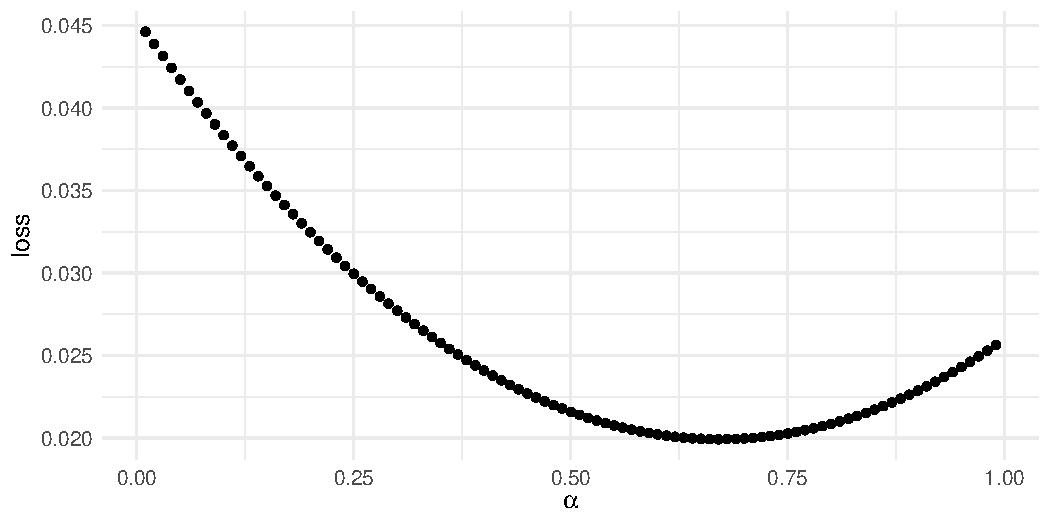
\includegraphics[width=\maxwidth]{figure/cv_benchmark-1} 

}

\caption[Out of sample variance estimates from the 5-fold cross validation]{Out of sample variance estimates from the 5-fold cross validation.}\label{fig:cv_benchmark}
\end{figure}

\end{knitrout}

In Figure \ref{fig:cv_benchmark} we illustrate the out of sample variance aggregated over folds. 
Cross validation suggest that the optimal value should be $0.68$. 
The analytic method from \citet{bodnar2018estimation} suggests that the optimal value is $0.7968$.
The "correct" value of $\alpha$, as given by the oracle estimator, is equal to $0.8151$. 
Its limiting value (see Theorem 2.1 \citet{bodnar2018estimation}) is equal to $0.7933$.
Although none of the methods are spot on, the bona-fide estimator is closer to what the optimal value should be.
Furthermore, changing the number of folds in the K-fold cross validation can give quite different results in what the optimal value should be.
This linear shrinkage approach is used in Paper \ref{sec:paper3} through \ref{sec:paper5}.

So far we have limited our approach to shrinking the weights. 
The next step is to shrink the elements of $\bS$.
If we do so then we can consider the case where $c>1$.
We leave this as an open question for the next section where we describe the papers in more detail.
%\begin{enumerate}
%	\item Other types of estimators and why they might be better than $\bS$.
%	\item Rotation-invariant estimation - what does it mean (we do not want to target eigenvectors)?
%\end{enumerate}

%%%%%% ------------------------------------------------------------------------
\chapter{Summary of papers}\label{ch:papersummary}
%%%%%% ------------------------------------------------------------------------


The papers presented here are among a total of ... papers produced. These are selected based their common theme.

\section{Paper 1 - Sampling Distributions of Optimal Portfolio Weights and Characteristics in Small and Large Dimensions}\label{sec:paper1}
The paper investigates a fundamental question in modern portfolio theory. 
What are the actual implications of using the sample covariance matrix $\bS$ and the sample mean $\byb$ instead of the true covariance matrix $\bSigma$ and $\bmu$?
The paper does so when the returns follow a multivariate normal distribution. 
In it we derive the distribution for all optimal portfolios on the common form
\begin{equation}\label{eqn:paper1_eq1}
  \bL\hbw_{opt} = \bL\hbw_{GMV} + g(\hR, \hV, \hs)\bL\hat{\bQ}\byb
\end{equation}
for some matrix $\bL$ of size $k \times p$ where $k<p$.
To do so, we derive the stochastic representation for the joint distribution of all quantities in the equation \eqref{eqn:paper1_eq1}. 
That enables us to efficiently simulate from the distribution.
Using this representation we can easily compute quantiles of the joint distribution of the efficient frontier.
Furthermore, we also derive the high-dimensional asymptotic distribution of said joint distribution. 
The high-dimensional asymptotic distribution is then compared to different models.
One scenario considers simulations from the stochastic representation, trying to deduce the finite-sample properties.
The other scenarios try to investigate what happens when we deviate from the model.
As one can expect, the high-dimensional distribution works well under the assumptions though seem to be reasonably robust from deviations of the model.
The hardest part to determine is what different characteristics of the return distribution have on the sample distribution of the quantities in \eqref{eqn:paper1_eq1} it remains an unanswered question.

\section{Paper 2 -Tangency portfolio weights under a skew-normal model in small and large dimensions}\label{sec:paper2}
In this paper we investigate a portfolio from chapter \ref{ch:MPT}, the tangency portfolio. 
The portfolio was obtained from the quadratic utility function, namely
\begin{equation}
  \min_{\bw} \bw^\top (\bmu -r_f\ones) - \frac{\gamma}{2} \bw^\top \bSigma \bw
\end{equation}
This paper extends Paper 1 as it considers investments in a risk-free asset and use an extension of the multivariate normal model, the CSN model presented in chapter \ref{ch:estim}. 
The model can include skewness in the asset returns, a trait they usually exhibit (see e.g. \citet{cont2001empirical}). 
Similarly to Paper 1, we derive the distribution of the sample tangency portfolio.
We investigate what implications the model has on the sample tangency portfolio.
In short, skewness results in a bias of the portfolio weights. 
The investor will not hold the correct portfolio on average.
Furthermore, we also investigate its high-dimensional distribution and show that the skewness disappears asymptotically. 
The high-dimensional distribution is the same as the previous research have shown (see .e.g. \citet{karlsson2021statistical})

\section{Paper 3 - Dynamic Shrinkage Estimation of the High-Dimensional Minimum-Variance Portfolio}\label{sec:paper3}
This paper solves a practical feature when investing in the GMV portfolio: how to rebalance it at fixed time points. 
If the investor owns a GMV portfolio and waits for a week, month or year the data will likely indicate that they should hold another portfolio than what they are.
The change can be quite large if $n$ is sufficiently small.
A natural question to ask is how to go from one portfolio to another, e.g. how to rebalance optimally when we receive a new set of data. 

In this paper we develop a dynamic rebalancing scheme for the GMV portfolio. 
It aims to decrease the out-of-sample variance between the holding portfolio, which might be a random GMV portfolio, and the GMV portfolio that you are supposed to hold given the data you see. 
We consider portfolios on the following form
\begin{equation}
  \hbw_{SH;n_{i}}=\psi_{i}\hbw_{S;n_i}+ (1-\psi_{i})\hbw_{SH;n_{i-1}},
\end{equation}
where $\hbw_{S;n_i}$, $i=1,2,...,T$, is the Traditional sample GMV portfolio using the $i$th sample of size $n_i$ to estimate the GMV portfolio weights in \eqref{eqn:GMV}. 
The initial portfolio, $\hbw_{SH;0}$, can be a random GMV portfolio or a deterministic target portfolio $\bb$.
We assume that the investor have specified fixed dates $t_i$, $i=1,2,...,T$ that they want to rebalance their GMV portfolio. 
The shrinkage coefficients are then determined through the following optimization problem
$$
\min_{\psi_i} \hbw_{SH;n_{i}}^\top \bSigma \hbw_{SH;n_{i}}.
$$
The problem is similar to the linear shrinkage discussed in chapter \ref{ch:highdim}.
It is an extension to the work of \citet{bodnar2018estimation} and use the flexible location and scale model discussed in \eqref{eqn:location_scale_model}.

The portfolio is shown to produce great results in an extensive simulation study.
It also provides a better estimator for the volatility in comparison to the Traditional sample GMV as well as the GMV portfolio using \citet{lw20} nonlinear shrinkage estimator for the sample covariance matrix.
There are also many other benefits of using the portfolio strategy.
To transition from one portfolio to the next costs money.
That will diminish the return and profit you make.
Furthermore, its not always possible to go from one portfolio to the next in a day or even a month.
The traditional GMV portfolio might suggest that an institution should first own a large long position and the next month a large short position.
Depending on the size of that institutions portfolio and the size of these positional changes, that might be illegal. 
It can be deemed market influencing or just outright impossible to sell that many assets, there is a liquidity issue.

\section{Paper 4 - Is the empirical out-of-sample variance an informative risk measure for high-dimensional portfolios}\label{sec:paper4}
Any empirical application using the GMV portfolio is bound to include the volatility or variance as a performance measure. 
A natural question to ask is then: is the empirical out-of-sample variance a consistent estimator of the variance? 
Furthermore, is it a good option to use or are there perhaps better options to use as performance measures? 
In this paper we investigate two different metrics of evaluation that are common to the GMV portfolio, the out-of-sample variance and the relative out-of-sample loss.   

We consider the location and scale model from \eqref{eqn:location_scale_model} and three different portfolios. 
The first portfolio is the Traditional GMV portfolio from \eqref{eqn:GMV}, the second is the portfolio from \citet{bodnar2018estimation} and the last is the linear shrinkage portfolio from \citet{frahm2010}.
For the three different portfolios we derive their out-of-sample variance, relative loss and their empirical counterparts. 
We do so under different assumptions on the parameters of the model.
Most notably, there is a natural ordering to the different out-of-sample losses.
The empirical out-of-sample loss is smallest for \citet{bodnar2018estimation}, second to smallest is \citet{frahm2010} and the largest is the traditional sample GMV portfolio.
Furthermore, we are able to derive the empirical out-of-sample variance for the different portfolios.
The assumptions that are necessary for convergence of the empirical out-of-sample variance are quite different from those used for the empirical out-of-sample loss.
We argue that the assumptions necessary for convergence of the empirical out-of-sample variance are stronger than the empirical out-of-sample loss.
The theoretical findings are investigated in a simulations study where we see an indication to that the ordering will always hold even when the model assumptions are violated.

\section{Paper 5 - Double shrinkage}\label{sec:paper5}
In this thesis we mostly use $\bS$ and cope with that the sample covariance matrix is a noisy estimator by linear shrinkage or understanding the uncertainty it provides.
Using this estimator has implied that we have only consider $c<1$.
In this paper we use a version of Thikonov shrinkage on the sample covariance matrix as well as the linear shrinkage from previous papers. 
That enables us to cover the case where $c>1$ and potentially create a more robust estimator of the portfolio weights.
In this paper we consider the following shrinkage estimator
$$
\hbw_{SH} = \psi \frac{\left(\bS + \lambda \bI_p \right)^{-1}\ones_p}{\ones_p^\top\left(\bS + \lambda \bI_p \right)^{-1}\ones_p} + (1-\psi)\bb.
$$
As previously, since we are dealing with the GMV portfolio we naturally use the out-of-sample variance to determine $\psi$ and $\lambda$.
It turns out that we can not construct a closed-form oracle estimator for the shrinkage parameters.
However, we are able to construct an oracle loss function, which we can then derive a bona-fide estimator for.
The bona-fide loss is consistent of the oracle loss.

The model is seen to perform on-par with the nonlinear shrinkage of \citet{lw20} in all simulations and beat their method in a empirical analysis.
Furthermore, it also increases/decreases the results of several other portfolio metrics.
\textbf{more comments...}

%\section*{Paper 6 - The capital market line, tangency portfolio and the effect of Tikhonov regularization in higher dimensions}\label{sec:paper6}

\section{Other research results}

Paper \ref{sec:paper3} is accompanied by the R-package \citet{DOSPortfolio}, available on CRAN. 
The readers are free, or rather encouraged(!), to install it with \hlkwd{install.packages}\hlstd{(}\hlstr{"DOSPortfolio"}\hlstd{)}. 
The package provides a simple interface for the methods implemented in the paper. 
In \ref{DOSportfolio} we display a short example on how to construct the dynamic portfolio weights. 
The package is the first iteration of possibly many more portfolios which can be constructed in a similar fashion.
\begin{knitrout}\small
\definecolor{shadecolor}{rgb}{1, 1, 1}\color{fgcolor}\begin{kframe}
\captionof{chunk}{R-code which showcase the use of the DOSPortfolio package.}\label{DOSportfolio}\begin{alltt}
\hlkwd{library}\hlstd{(DOSPortfolio)}
\hlstd{df} \hlkwb{<-} \hlkwd{read_csv}\hlstd{(}\hlstr{"../data/returns.csv"}\hlstd{)}
\hlstd{p} \hlkwb{<-} \hlnum{350}\hlstd{; n} \hlkwb{<-} \hlnum{400}
\hlcom{# Sample p assets}
\hlkwd{set.seed}\hlstd{(}\hlnum{1234}\hlstd{)}
\hlstd{asset_cols} \hlkwb{<-} \hlkwd{sample}\hlstd{(}\hlnum{2}\hlopt{:}\hlkwd{ncol}\hlstd{(df),} \hlkwc{size} \hlstd{= p)}
\hlcom{# specify reallocation points}
\hlstd{reallocation_points} \hlkwb{<-} \hlkwd{seq}\hlstd{(n,} \hlkwd{nrow}\hlstd{(df),} \hlkwc{by}\hlstd{=n)}
\hlcom{# estimate portfolio weights}
\hlstd{dos_weights} \hlkwb{<-} \hlstd{df} \hlopt
  \hlkwd{select}\hlstd{(}\hlkwd{all_of}\hlstd{(asset_cols),} \hlopt{-}\hlstd{date)} \hlopt
  \hlkwd{DOSPortfolio}\hlstd{(.,}
               \hlkwc{reallocation_points} \hlstd{= reallocation_points,}
               \hlkwc{target_portfolio} \hlstd{=} \hlkwd{rep}\hlstd{(}\hlnum{1}\hlstd{,} \hlkwd{ncol}\hlstd{(.))}\hlopt{/}\hlkwd{ncol}\hlstd{(.),}
               \hlkwc{shrinkage_type} \hlstd{=} \hlstr{"overlapping"}\hlstd{)}
\end{alltt}
\end{kframe}
\end{knitrout}
Furthermore, the following papers were also coauthored throughout the writing of this thesis \cite{bodnar2020quantile}, \cite{bodnar2021bayesian}  and \cite{bodnar2021quantile}.
The first presents an analytic derivation of the MPT framework in the Bayesian setting. 
It specifically looks at how quantiles of optimal portfolios can be constructed and the effects of estimation uncertainty in these. 
This is especially important since the regulations in place demands that you report quantile-based risk measures (see \citet{basel4}).
The second paper provides a continuation on the first. 
The idea is to model the belief of the investor explicitly and to construct a prior which captures what the likelihood cannot. 
We impose a prior distribution which adapts to the recent observations when the market is turbulent. 
The algorithm is seen to work well when markets are turbulent.
The third paper also considers quantile based portfolios. 
It does so in a general framework, not necessarily as the same framework as MPT where we only use the first two moments of the return distribution.



%%%%%% ------------------------------------------------------------------------
\chapter{Future research}\label{ch:future}
%%%%%% ------------------------------------------------------------------------


There are many possible extensions and future projects to the thesis at hand.
We talk very much of estimation uncertainty and how to cope with it.
Bayesian statistics provide a straightforward way to integrate that. 
However, it demands indepth knowledge of MCMC and also how to construct good prior distributions.
Neither are easy tasks.
Another approach of incorporating estimation uncertainty is robust optimization.
Robust optimization, in a MPT setting, tries to incorporate the estimation uncertainty into the portfolio allocation problem itself.
The literature is large. 
Are there connections to be made and especially with Empirical Bayes?

In Paper \ref{sec:paper3} we consider the allocations points fixed.
That assumption can be limiting for some investors.
Can we incorporate that decision process into the portfolio allocation problem?

Many Multivariate GARCH models can be formulated as the following BEKK model (see e.g. \citet{engle1995multivariate})
\begin{equation}\label{eqn:BEKK}
  \bH_t = \bC \bC^\top + \sum_{k=1}^K \bA_k \boldsymbol{\epsilon}_{t-1}\boldsymbol{\epsilon}_{t-1}^\top \bA_k^\top + \sum_{k=1}^K \bG_k \bH_{t-1}\bG_k^\top,
\end{equation}
where $\bH_i$ is a sequence of conditional covariance matrices, $\boldsymbol{\epsilon}_t | \mathcal{F}_{t-1} \sim N_p(\mathbf{0], \bH_t})$ and the matrices $\bC, \bA_i$ and $\bG_i$ are of appropriate dimensions.
These are usually very hard to fit and use for portfolio allocations. 
The first issue is due to the number of parameters in the model.
One parametrization is that $\tilde \bC = \bC\bC^\top$, where $\tilde \bC > 0$, then $\bC$ can be any matrix square root with up to $p(p-1)/2$ parameters to estimate. 
Furthermore, the constraint that its product should be positive definite is highly nonlinear and can be hard to suffice.
Using the same argument for each of the matrices we have $(K+1/2)p(p-1)$ parameters to estimate. 
Building a portfolio of size 10 with $K=1$ implies that we need to estimate $135$ parameters.
Furthermore, although the constraints should enforce forecasts which are positive definite its not necessarily true that they will numerically be invertible.
They can provide forecasts which are very close to singular.
The first issue can be solved if one can formulate the models as Recurrent Neural Networks and use deep-learning libraries Torch or Tensorflow to fit the models. 
These are tailored to solve the problem of fitting very large models! 
Recent large Natural Languange Processing models have \textit{billions} of parameters (see e.g. \citet{brown2020language}). 
By placing BEKK models in this framework one also has the possibility to develop new models. 
The development is solely determined by constructing new layers to the networks. 
It would also be easier to integrate different sources of information in the models.

\printbibliography
%%%%%%%%%%%%%%%%%%%%%%%%%%%%%%%%%%%%%%%%%%
% Insert papers here
%%%%%%%%%%%%%%%%%%%%%%%%%%%%%%%%%%%%%%%%%%

\end{document}
